% \ll --> compile
% \lv --> view

\documentclass[a4paper]{article}
%-----------------------------
% preamble
%-----------------------------
\usepackage[sumlimits,]{amsmath}
\usepackage[utf8]{inputenc}
\usepackage[english]{babel}
\usepackage{graphicx}
\usepackage{subcaption}
\usepackage{hyperref}
\usepackage{float}
%\usepackage[document]{ragged2e}

\graphicspath{ 
    {../figures/} 
    {../figures/theoretical-ex/} 
    {../figures/pre-ex1/} 
    {../figures/pre-ex2/} 
    {../figures/ex1/} 
    {../figures/ex2/} 
}

%-----------------------------
% body
%-----------------------------
\begin{document}

\begin{figure}
    \centering
    % UNICAMP logo
    \begin{subfigure}{0.45\textwidth}
        \centering
        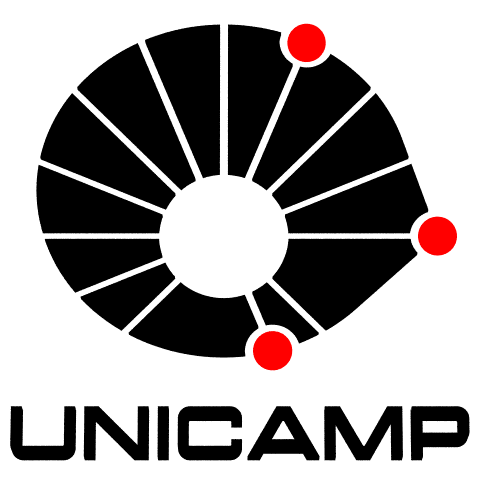
\includegraphics[width=1.5cm]{unicamp}
        \label{fig:unicamp}
    \end{subfigure}
    \hfill
    % FEEC logo
    \begin{subfigure}{0.45\textwidth}
        \centering
        
\includegraphics[width=1.5cm]{feec}
        \label{fig:feec}
    \end{subfigure}
    % caption and label
%    \caption{Folds used in cross-validation}
%    \label{fig:pre-ex1-kfold}
\end{figure}

\title{EFC1 - Exercise 1}
\author{Rafael Claro Ito}
%R.A.: 118430
%ito.rafael@gmail.com
\date{September 2019}
\maketitle
\newpage

%=================================================
\section{Theoretical Activities}
%=================================================

%=======================================
\subsection{Exercise 1}
%=======================================

%==============================
\subsubsection{a) Obtain P(X) e P(Y).}
%==============================

%------------------------
% P_X(0)
\paragraph{$i) \; P_X(0):                       $
\\
$ \displaystyle P_X(0) = \sum_{y} P_{XY}(0,y)   $\\
$ P_X(0) = P_{XY}(0,0) + P_{XY}(0,1)            $\\
$ P_X(0) = 1/6 + 3/8                            $\\
$ \boxed{ P_X(0) = 13/24 }                      $\\
}
%------------------------
% P_X(1)
\paragraph{$ii) \; P_X(1):                      $
\\
$ \displaystyle P_X(1) = \sum_{y} P_{XY}(1,y)   $\\
$ P_X(1) = P_{XY}(1,0) + P_{XY}(1,1)            $\\
$ P_X(1) = 1/8 + 1/3                            $\\
$ \boxed{ P_X(1) = 11/24 }                      $\\
}
%------------------------
% P_Y(0)
\paragraph{$iii) \; P_Y(0):                     $
\\
$ \displaystyle P_Y(0) = \sum_{x} P_{XY}(x,0)   $\\
$ P_Y(0) = P_{XY}(0,0) + P_{XY}(1,0)            $\\
$ P_Y(0) = 1/6 + 1/8                            $\\
$ \boxed{ P_Y(0) = 7/24 }                       $\\
}
%------------------------
% P_Y(1)
\paragraph{$iv) \; P_Y(1):                      $
\\
$ \displaystyle P_Y(1) = \sum_{x} P_{XY}(x,1)   $\\
$ P_Y(1) = P_{XY}(0,1) + P_{XY}(1,1)            $\\
$ P_Y(1) = 3/8 + 1/3                            $\\
$ \boxed{ P_Y(1) = 17/24 }                      $\\
}

%==============================
\subsubsection{b) Calculate P(X = 0$|$Y = 0).}
%==============================
% P(X=0|Y=0)
\paragraph{
$ \displaystyle P_{X|Y}(x,y) = \frac{P_{XY}(x,y)}{P_Y(y)}   $\\
$ \displaystyle P_{X|Y}(0,0) = \frac{P_{XY}(0,0)}{P_Y(0)}   $\\
$ P_{X|Y}(0,0) = \frac{1/6}{7/24}                           $\\
$ \boxed{ P_{X|Y}(0,0) = 4/7 }                              $\\
}

%==============================
\subsubsection{c) Calculate E[X] e E[Y].}
%==============================

%------------------------
% E[X]
\paragraph{$ i) \; E[X]:                       $
\\
$ \displaystyle E[X] = \sum_{k} x_k P_X(x_k)   $\\
$ E[X] = 0 \cdot P_X(0) + 1 \cdot P_X(1)       $\\
$ \boxed{ E[X] = 11/24 }                       $\\
}
%------------------------
% E[Y]
\paragraph{$ ii) \; E[Y]:                      $
\\
$ \displaystyle E[Y] = \sum_{k} y_k P_Y(y_k)   $\\
$ E[Y] = 0 \cdot P_Y(0) + 1 \cdot P_Y(1)       $\\
$ \boxed{ E[Y] = 17/24 }                       $\\
}

%==============================
\subsubsection{d) Are the variables independents? Why?}
%==============================
$ P_{XY}(0,0) \neq P_{X}(0) P_{Y}(0)                                $\\
$ \displaystyle \frac{1}{6} \neq \frac{13}{24} \cdot \frac{7}{24}   $\\

Since $P_{XY}(0,0) \neq P_{X}(0) P_{Y}(0)$, the variables X and Y are not independents.

%=======================================
\subsection{Exercise 2}
%=======================================

%==============================
\subsubsection{a) Calculate H(X), H(Y) e H(X$|$Y).}
%==============================

$ P_X(0) = P_{XY}(0,0) + P_{XY}(0,1) = 1/4     $\\
$ P_X(1) = P_{XY}(1,0) + P_{XY}(1,1) = 3/4     $\\
$ P_Y(0) = P_{XY}(0,0) + P_{XY}(1,0) = 3/8     $\\
$ P_Y(1) = P_{XY}(0,1) + P_{XY}(1,1) = 5/8     $\\

%------------------------
% H(X)
\paragraph{$ i) \; H(X):                                    $
\\
$ \displaystyle H(X) = -\sum_{x} p(x) \log_2 [p(x)]         $\\
$ H(X) = -P_X(0) \log_2 [P_X(0)] -P_X(1) \log_2 [P_X(1)]    $\\
$ \displaystyle 
    H(X) = - \frac{1}{4} \log_2 \left( \frac{1}{4} \right) 
           - \frac{3}{4} \log_2 \left( \frac{3}{4} \right)  $\\
$ H(X) = 0.5 + 0.3113                                       $\\
$ \boxed{ H(X) = 0.8113 }                                   $\\
}
%------------------------
% H(Y)
\paragraph{$ ii) \; H(Y):                                   $
\\
$ \displaystyle H(Y) = -\sum_{y} p(y) \log_2 [p(y)]         $\\
$ H(Y) = -P_Y(0) \log_2 [P_Y(0)] -P_Y(1) \log_2 [P_Y(1)]    $\\
$ \displaystyle 
    H(Y) = - \frac{3}{8} \log_2 \left( \frac{3}{8} \right) 
           - \frac{5}{8} \log_2 \left( \frac{5}{8} \right)  $\\
$ H(Y) = 0.5306 + 0.4238                                    $\\
$ \boxed{ H(Y) = 0.9544 }                                   $\\
}
%------------------------
% H(X,Y)
\paragraph{$ iii) \; H(X,Y):                                $
\\
$ \displaystyle 
    H(X,Y) = -\sum_x \sum_y p(x,y) \log_2 [p(x,y)]            $\\
$ H(X,Y) = - P_{XY}(0,0) \log_2 [P_{XY}(0,0)]                
         - P_{XY}(0,1) \log_2 [P_{XY}(0,1)] 
         - P_{XY}(1,0) \log_2 [P_{XY}(1,0)] 
         - P_{XY}(1,1) \log_2 [P_{XY}(1,1)]                 $\\
$ \displaystyle
    H(X,Y) = - 0 \cdot \log_2 (0)                              
          - \frac{1}{4} \log_2 \left( \frac{1}{4} \right)
          - \frac{3}{8} \log_2 \left( \frac{3}{8} \right)
          - \frac{3}{8} \log_2 \left( \frac{3}{8} \right)   $\\
$ H(X,Y) = 0 + 0.5 + 0.5306 + 0.5306                          $\\
$ \boxed{ H(X,Y) = 1.5613 }                                   $\\
}

%==============================
\subsubsection{b) Calculate H(X$|$Y) e H(Y$|$X).}
%==============================

%------------------------
% H(X|Y)
\paragraph{$ i) \; H(X|Y):      $
\\
$ H(X,Y) = H(Y) + H(X|Y)        $\\
$ H(X|Y) = H(X,Y) - H(Y)        $\\
$ H(X|Y) = 1.5613 - 0.9544      $\\
$ \boxed{ H(X|Y) = 0.6068 }     $\\
}
%------------------------
% H(Y|X)
\paragraph{$ ii) \; H(Y|X):     $
\\
$ H(X,Y) = H(X) + H(Y|X)        $\\
$ H(Y|X) = H(X,Y) - H(X)        $\\
$ H(Y|X) = 1.5613 - 0.8113      $\\
$ \boxed{ H(Y|X) = 0.75 }       $\\
}

%==============================
\subsubsection{c) Calculate I(X,Y).}
%==============================

$ I(X,Y) = H(X) - H(X|Y)        $\\
$ I(X,Y) = 0.8113 - 0.6068      $\\
$ \boxed{ I(X,Y) = 0.2044 }     $\\
\\
$ I(X,Y) = H(Y) - H(Y|X)        $\\
$ I(X,Y) = 0.9544 - 0.75        $\\
$ \boxed{ I(X,Y) = 0.2044 }     $\\

%=======================================
\subsection{Exercise 3}
%=======================================

$ C_1\sim\mathcal{N}(-1,1)      $\\
$ \mu_1 = -1                    $\\
$ \sigma_1 = 1                  $\\
\\
$ C_2\sim\mathcal{N}(1,1)       $\\
$ \mu_2 = 1                     $\\
$ \sigma_2 = 1                  $\\

%==============================
\subsubsection{a) Under the ML criteria, we have that x belongs to the class \texorpdfstring{$C_1$ if $p(x|C_1) > p(x|C_2)$}{C1 if p(x|C1) > p(x|C2)}:}
%==============================

$$ p(x|C_1) > p(x|C_2) $$

$$ \frac{1}{\sqrt{2\pi\sigma_1^2}}exp\left(-\frac{(x-\mu_1)^2}{2 \sigma_1^2}\right) > \frac{1}{\sqrt{2\pi\sigma_2^2}}exp\left(-\frac{(x-\mu_2)^2}{2 \sigma_2^2}\right) $$

$$ \frac{1}{\sqrt{2\pi\cdot1^2}}exp\left(-\frac{(x-(-1))^2}{2\cdot1^2}\right) > \frac{1}{\sqrt{2\pi\cdot1^2}}exp\left(-\frac{(x-1)^2}{2\cdot1^2}\right) $$

$$ exp\left(-\frac{(x+1)^2}{2}\right) > exp\left(-\frac{(x-1)^2}{2}\right) $$

$$ -(x+1)^2 > -(x-1)^2      $$
$$ -x^2-2x-1^2 > -x^2+2x-1  $$
$$ -2x > 2x                 $$
$$ \boxed{x < 0}            $$

\begin{figure}[h]
    \centering
    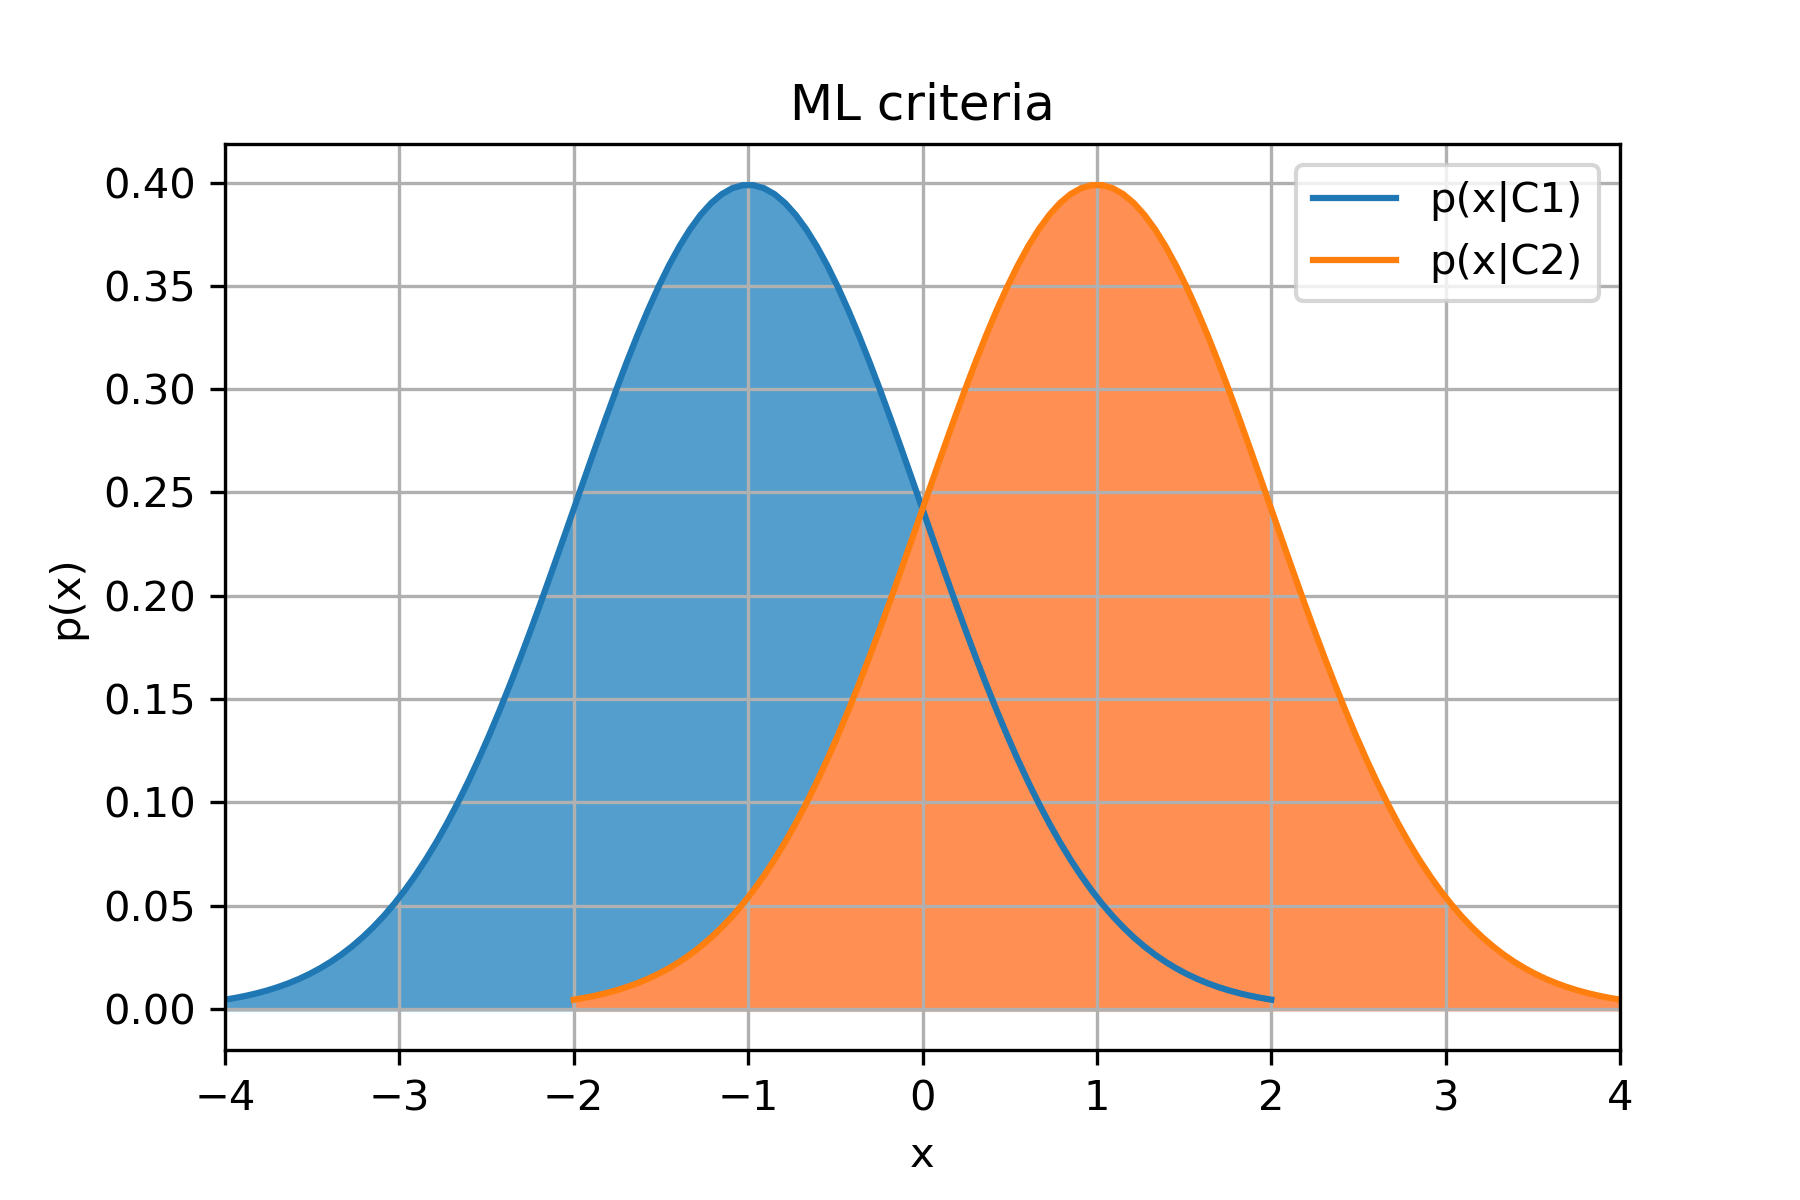
\includegraphics[width=12cm]{ML}
    \caption{Visualization of C1 and C2 distributions under the ML criteria}
    \label{fig:ML}
\end{figure}

As we can see in the figure \ref{fig:ML}, for x $<$ 0 the class C1 will be chosen.

%==============================
\subsection{b) Under the MAP criteria, we have that x belongs to the class $C_1$ if $p(C_1|x) > p(C_2|x)$:}
%==============================

$$ p(C_1) = 0.7 $$
$$ p(C_2) = 0.3 $$

$$ p(C_1|x) > p(C_2|x) $$

Applying Bayes' rule, we have:

$$ \frac{p(x|C_1)\cdot p(C_1)}{p(x)} > \frac{p(x|C_2)\cdot p(C_2)}{p(x)} $$

$$ \frac{1}{\sqrt{2\pi\sigma_1^2}}exp\left(-\frac{(x-\mu_1)^2}{2 \sigma_1^2}\right)\cdot p(C_1) > \frac{1}{\sqrt{2\pi\sigma_2^2}}exp\left(-\frac{(x-\mu_2)^2}{2 \sigma_2^2}\right) \cdot p(C_2) $$

$$ \frac{1}{\sqrt{2\pi\cdot1^2}}exp\left(-\frac{(x-(-1))^2}{2\cdot1^2}\right) (0.7) > \frac{1}{\sqrt{2\pi\cdot1^2}}exp\left(-\frac{(x-1)^2}{2\cdot1^2}\right) (0.3) $$

$$ exp\left(-\frac{(x+1)^2}{2}\right) (0.7) > exp\left(-\frac{(x-1)^2}{2}\right) (0.3) $$

Taking the ln from both sides:

$$ -\frac{(x+1)^2}{2} + \ln(0.7) > -\frac{(x-1)^2}{2} + \ln(0.3) $$

$$ -x^2-2x-1 + 2\ln(0.7) > -x^2+2x-1 + 2\ln(0.3)    $$
$$ -2x + 2\ln(0.7) > 2x + 2\ln(0.3)                 $$
$$ -x + \ln(0.7) > x + \ln(0.3)                     $$
$$ 2x  < \ln(0.7) - \ln(0.3)                        $$
$$ x  < \frac{\ln(0.7) - \ln(0.3)}{2}               $$
$$ \boxed{x  < 0.4236}                              $$

\begin{figure}[h]
    \centering
    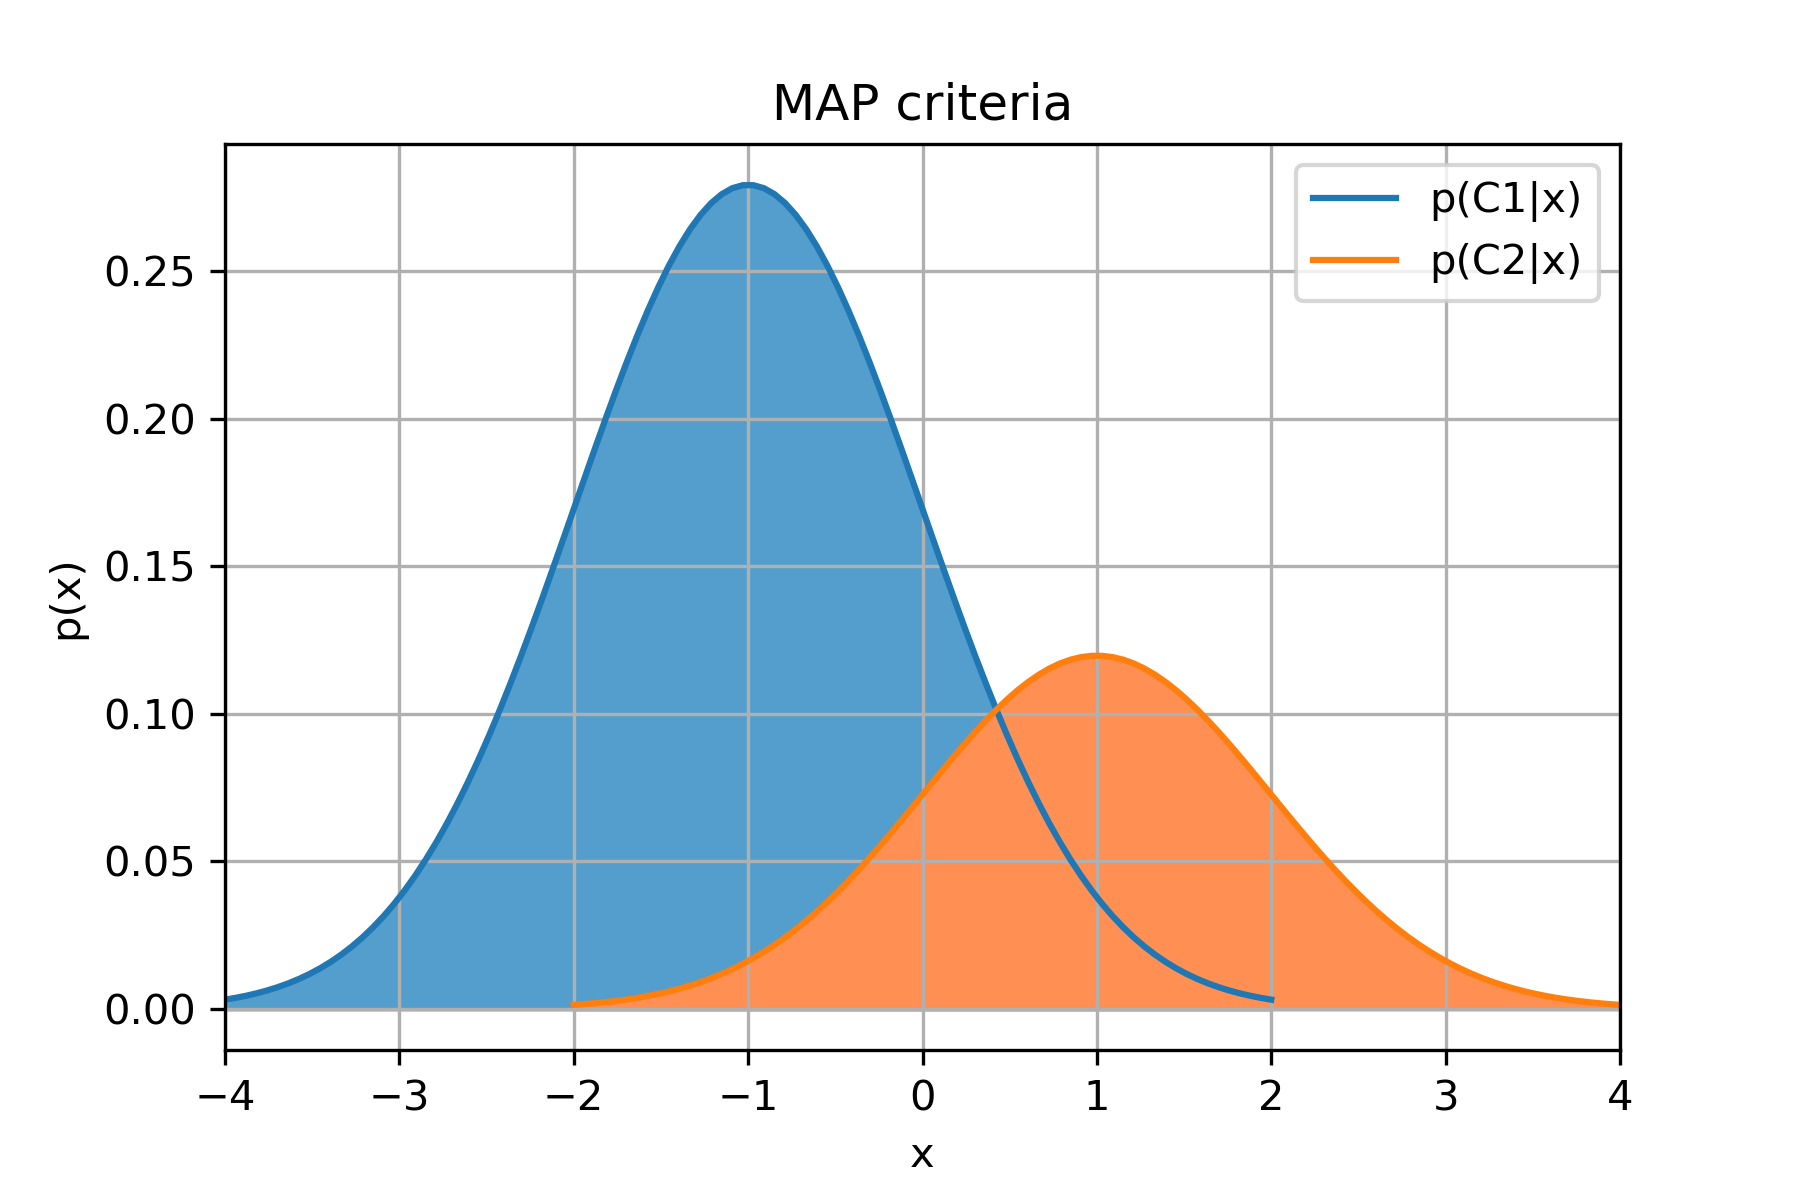
\includegraphics[width=12cm]{MAP}
    \caption{Visualization of C1 and C2 distributions under the MAP criteria}
    \label{fig:MAP}
\end{figure}

As we can see in the figure \ref{fig:MAP}, for x $<$ 0.4236 the class C1 will be chosen.
\newpage

%=================================================
\section{Computational Activities}
%=================================================

\paragraph{
All code presented and all figures showed here can be found at the following GitHub repository:\\
\url{https://github.com/ito-rafael/IA006C-MachineLearning}\\
In this repository, one can found the following files:\\
}

\begin{itemize}
    \item Jupyter Notebook
    \begin{itemize}
        \item \href{https://github.com/ito-rafael/IA006C-MachineLearning/blob/master/efc1/theoretical-ex.ipynb}{theoretical-ex.ipynb}
        \item \href{https://github.com/ito-rafael/IA006C-MachineLearning/blob/master/efc1/pre-ex1.ipynb}{pre-ex1.ipynb}
        \item \href{https://github.com/ito-rafael/IA006C-MachineLearning/blob/master/efc1/pre-ex2.ipynb}{pre-ex2.ipynb}
        \item \href{https://github.com/ito-rafael/IA006C-MachineLearning/blob/master/efc1/ex1.ipynb}{ex1.ipynb}
        \item \href{https://github.com/ito-rafael/IA006C-MachineLearning/blob/master/efc1/ex2.ipynb}{ex2.ipynb}
    \end{itemize}
    \item Python code
    \begin{itemize}
        \item \href{https://github.com/ito-rafael/IA006C-MachineLearning/blob/master/efc1/ex1.py}{ex1.py}
        \item \href{https://github.com/ito-rafael/IA006C-MachineLearning/blob/master/efc1/ex2.py}{ex2.py}
    \end{itemize}
    \item \LaTeX
    \begin{itemize}
        \item \href{https://github.com/ito-rafael/IA006C-MachineLearning/blob/master/efc1/LaTeX/efc1.tex}{efc1.tex}
    \end{itemize}
\end{itemize}

\paragraph{The notebook "theoretical-ex.ipynb" is used to generate the figures \ref{fig:ML} and \ref{fig:MAP}. The notebook "pre-ex1" is used only for data visualization. It shows how the dataset is split in order to use the k-fold cross-validation method. The notebook "pre-ex2" has a similar use than the previous one. It is used to visualize the data, but besides the raw data, it also plots the dataset linearly transformed before and after the application of the hyperbolic tangent function. The two last notebooks, "ex1" and "ex2" actually implements all the functions to train the models and that answers the exercises 1 and 2.}
\paragraph{The Python codes presented contain the same code of the notebooks. Finally, the \LaTeX file is the source code to generate this pdf.}

%=======================================
\subsection{Exercise 1}
%=======================================

\paragraph{The first thing we did before starting this exercise was to plot all the data, as can be seen in figure \ref{fig:pre-ex1-0}.}

\begin{figure}[H]
    \centering
    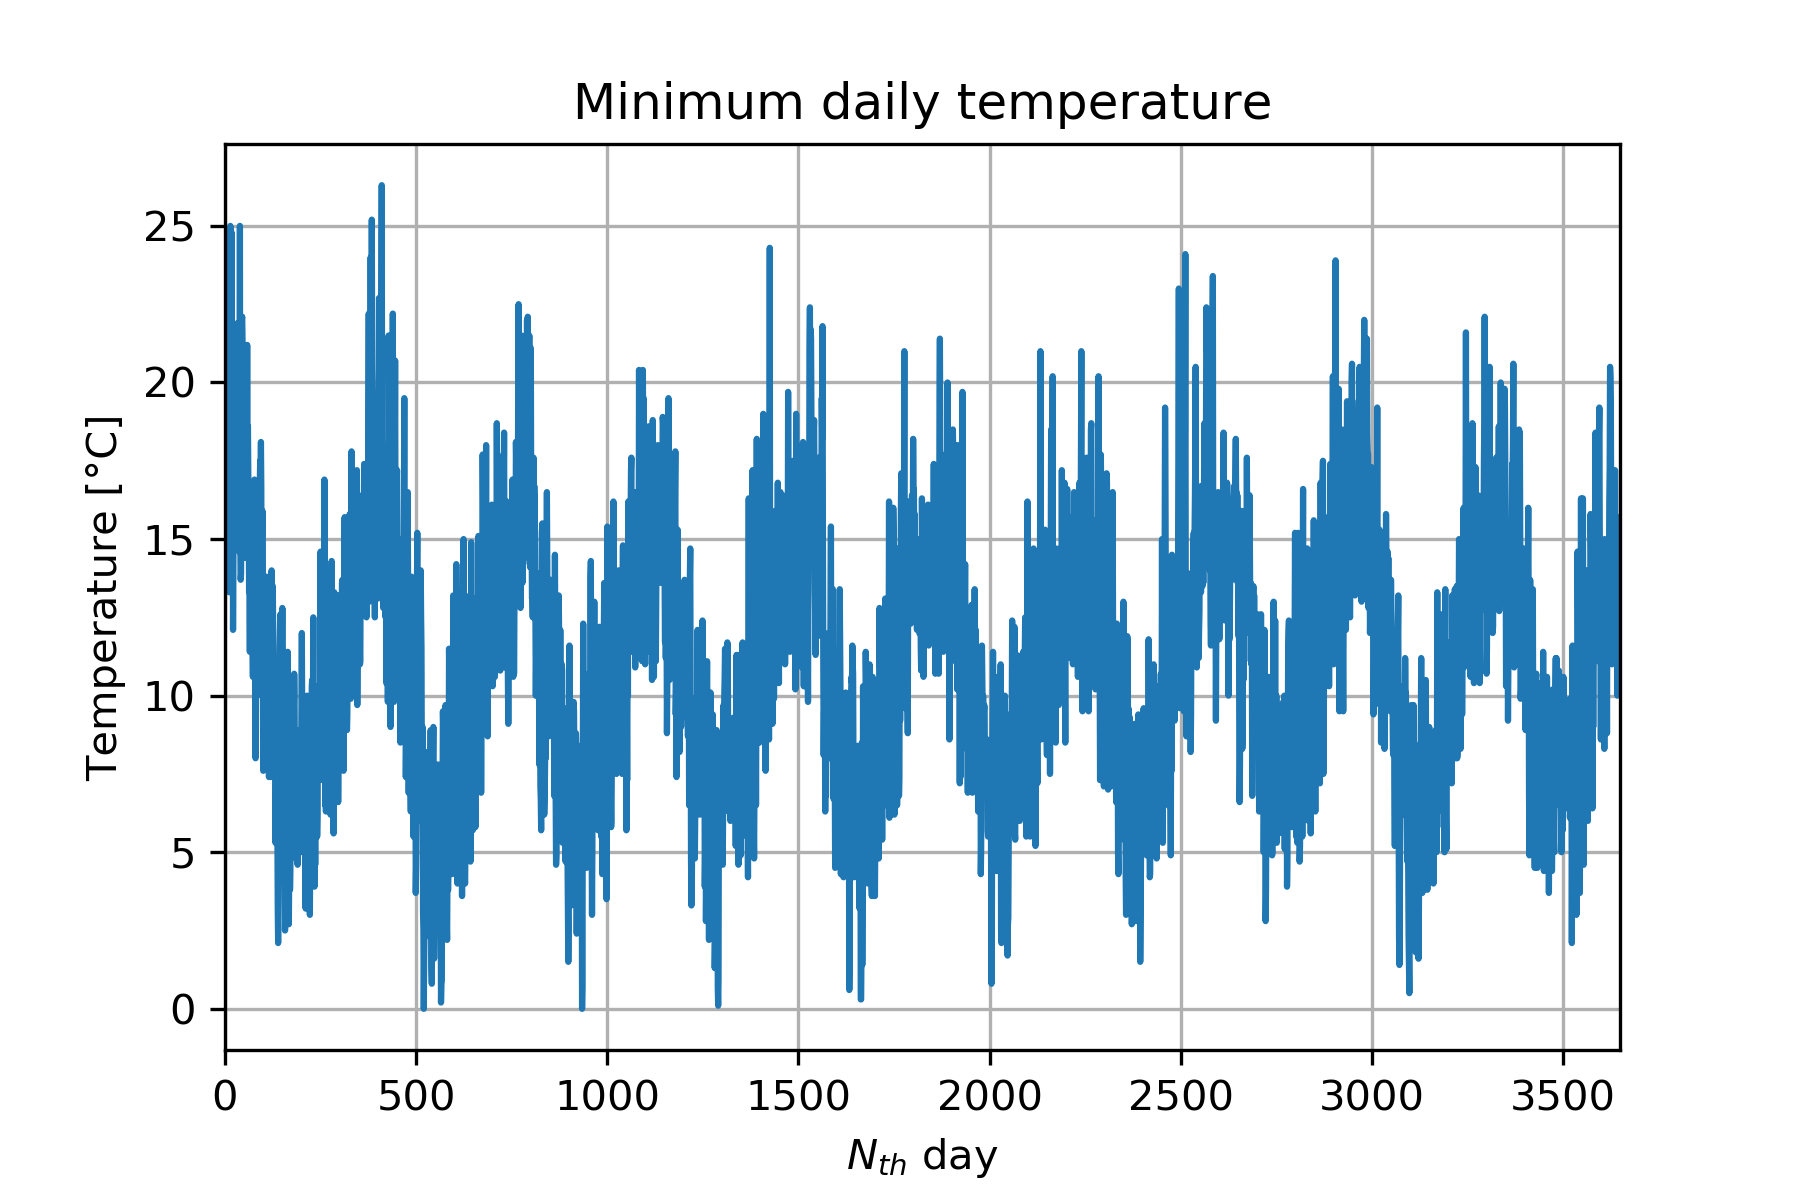
\includegraphics[width=12cm]{figure_0_all_data}
    \caption{All data}
    \label{fig:pre-ex1-0}
\end{figure}

\paragraph{The next step was to decide the number of folds used in the k-fold cross-validation method. Since we are treating a time series forecasting problem, it was decided to split the dataset equally to the number of the years of the dataset excluding the data used to test the model, so nine folds were used. When creating the folds, a method like the one that is showed in figure \ref{fig:pre-ex1-folds} was used.}

\begin{figure}[H]
    \centering
    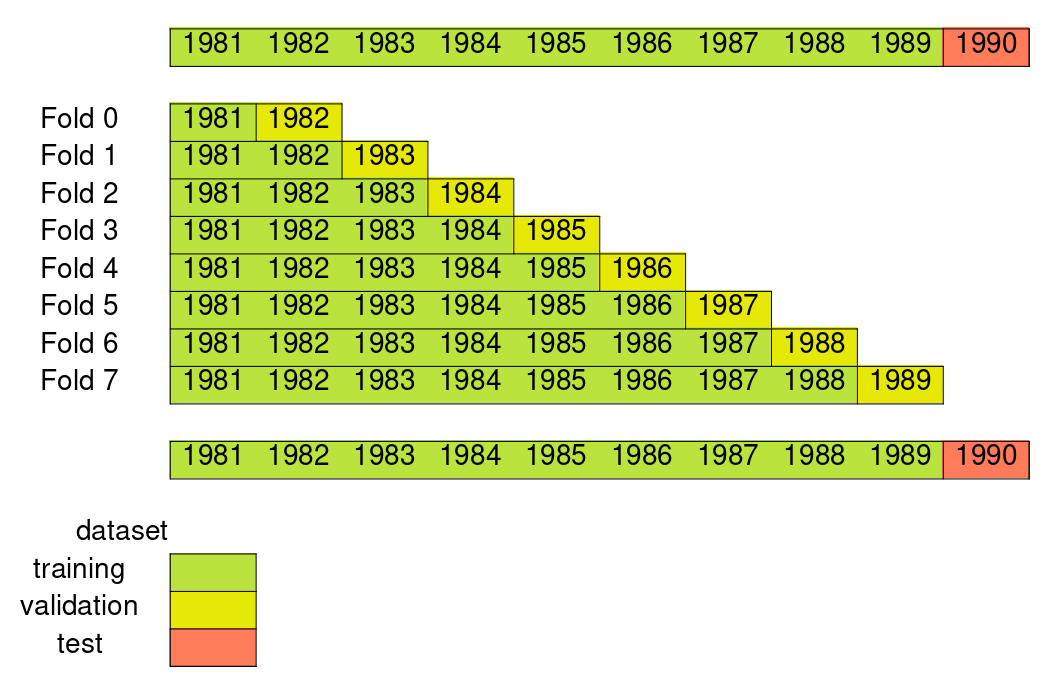
\includegraphics[width=12cm]{figure_0_kfold}
    \caption{Folds used to cross-validate the model}
    \label{fig:pre-ex1-folds}
\end{figure}

\paragraph{In this method, only past data is used to predict forward-looking data. The first fold is formed by only the first year of the dataset, the year 1981, while the year used at the validation step is the next year, 1982. The second fold uses all the data of the previous fold (train plus validation) as the data to be trained, and the next year, 1983, as the validation data. Doing this for all the folds we get the configuration showed in figure \ref{fig:pre-ex1-kfold}.}

\begin{figure}
    \centering
    % all data
    \begin{subfigure}{0.32\textwidth}
        \centering
        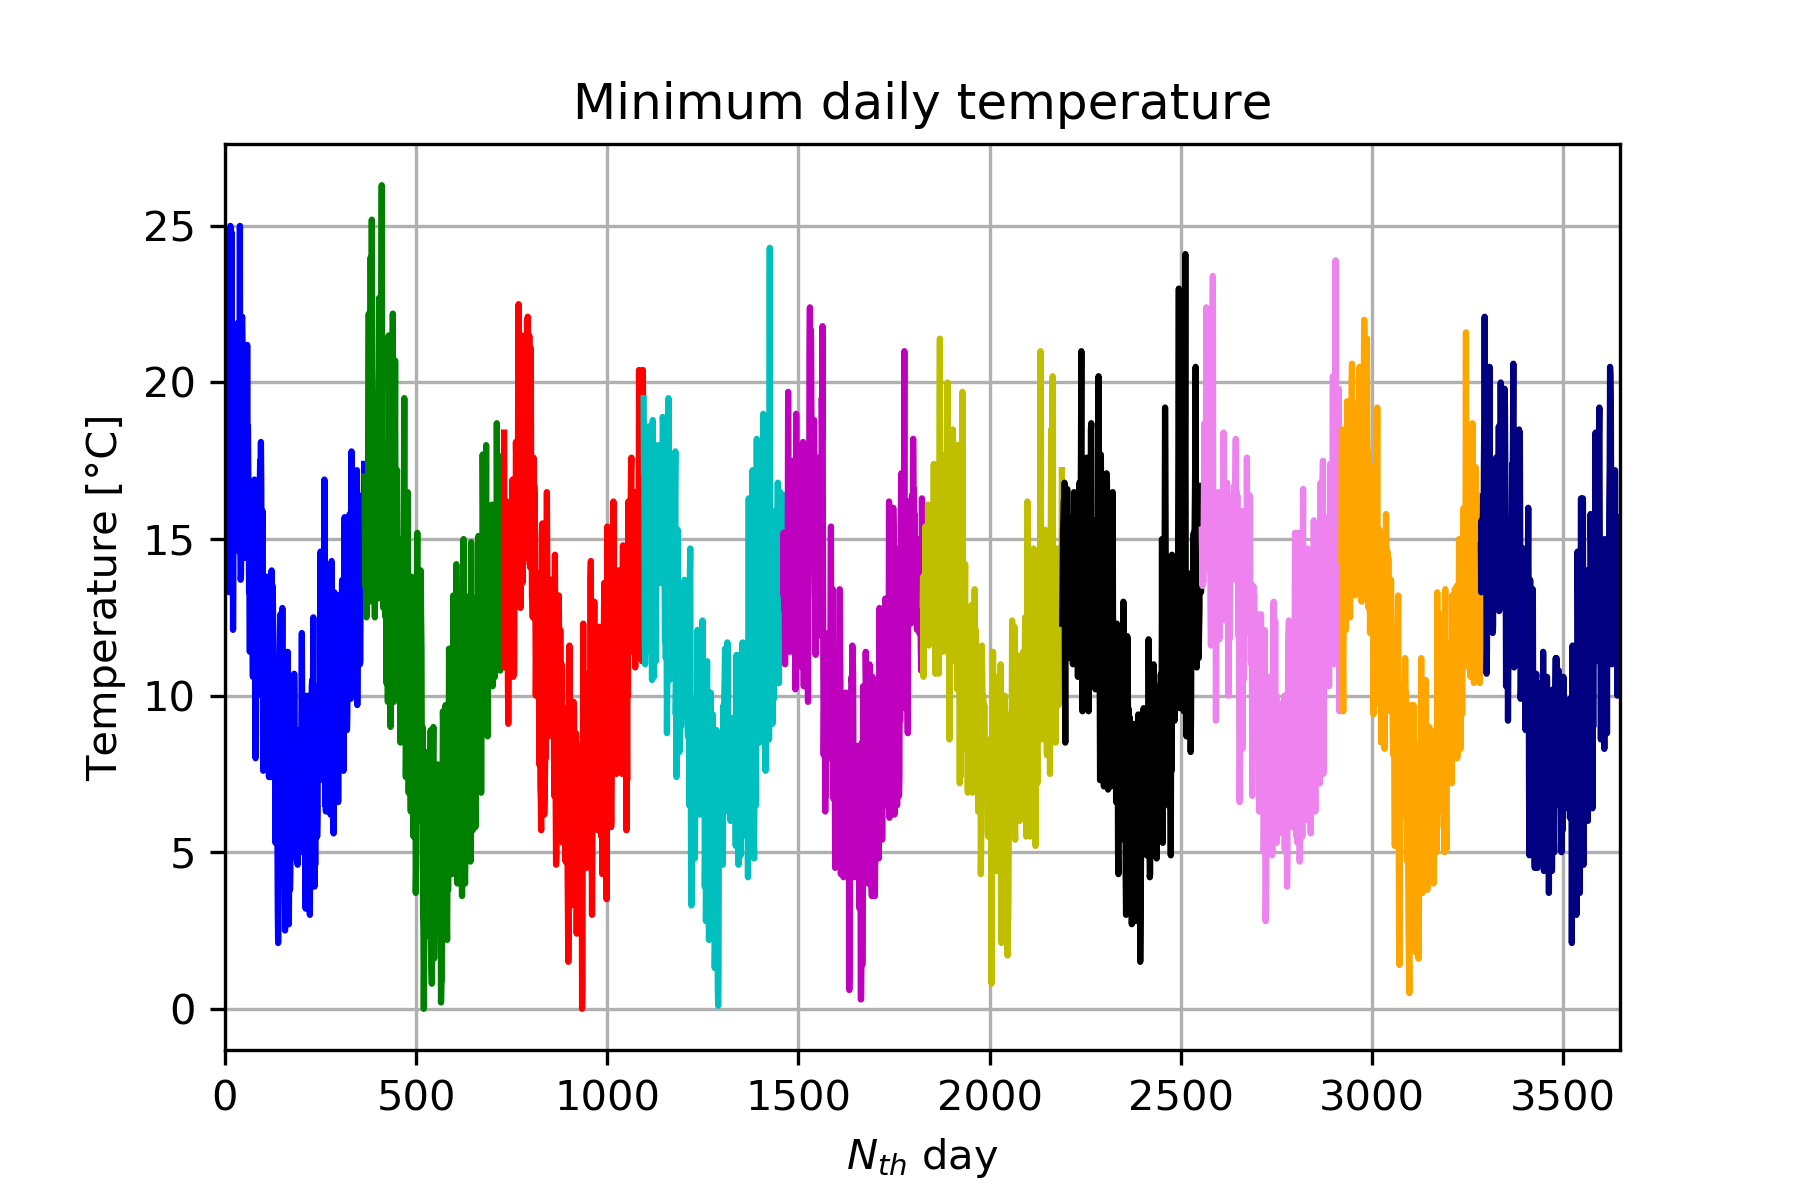
\includegraphics[width=3.85cm]{figure_1_data_split}
        \caption{Dataset split}
        \label{fig:sub1}
    \end{subfigure}
    \hfill
    % fold 1
    \begin{subfigure}{0.32\textwidth}
        \centering
        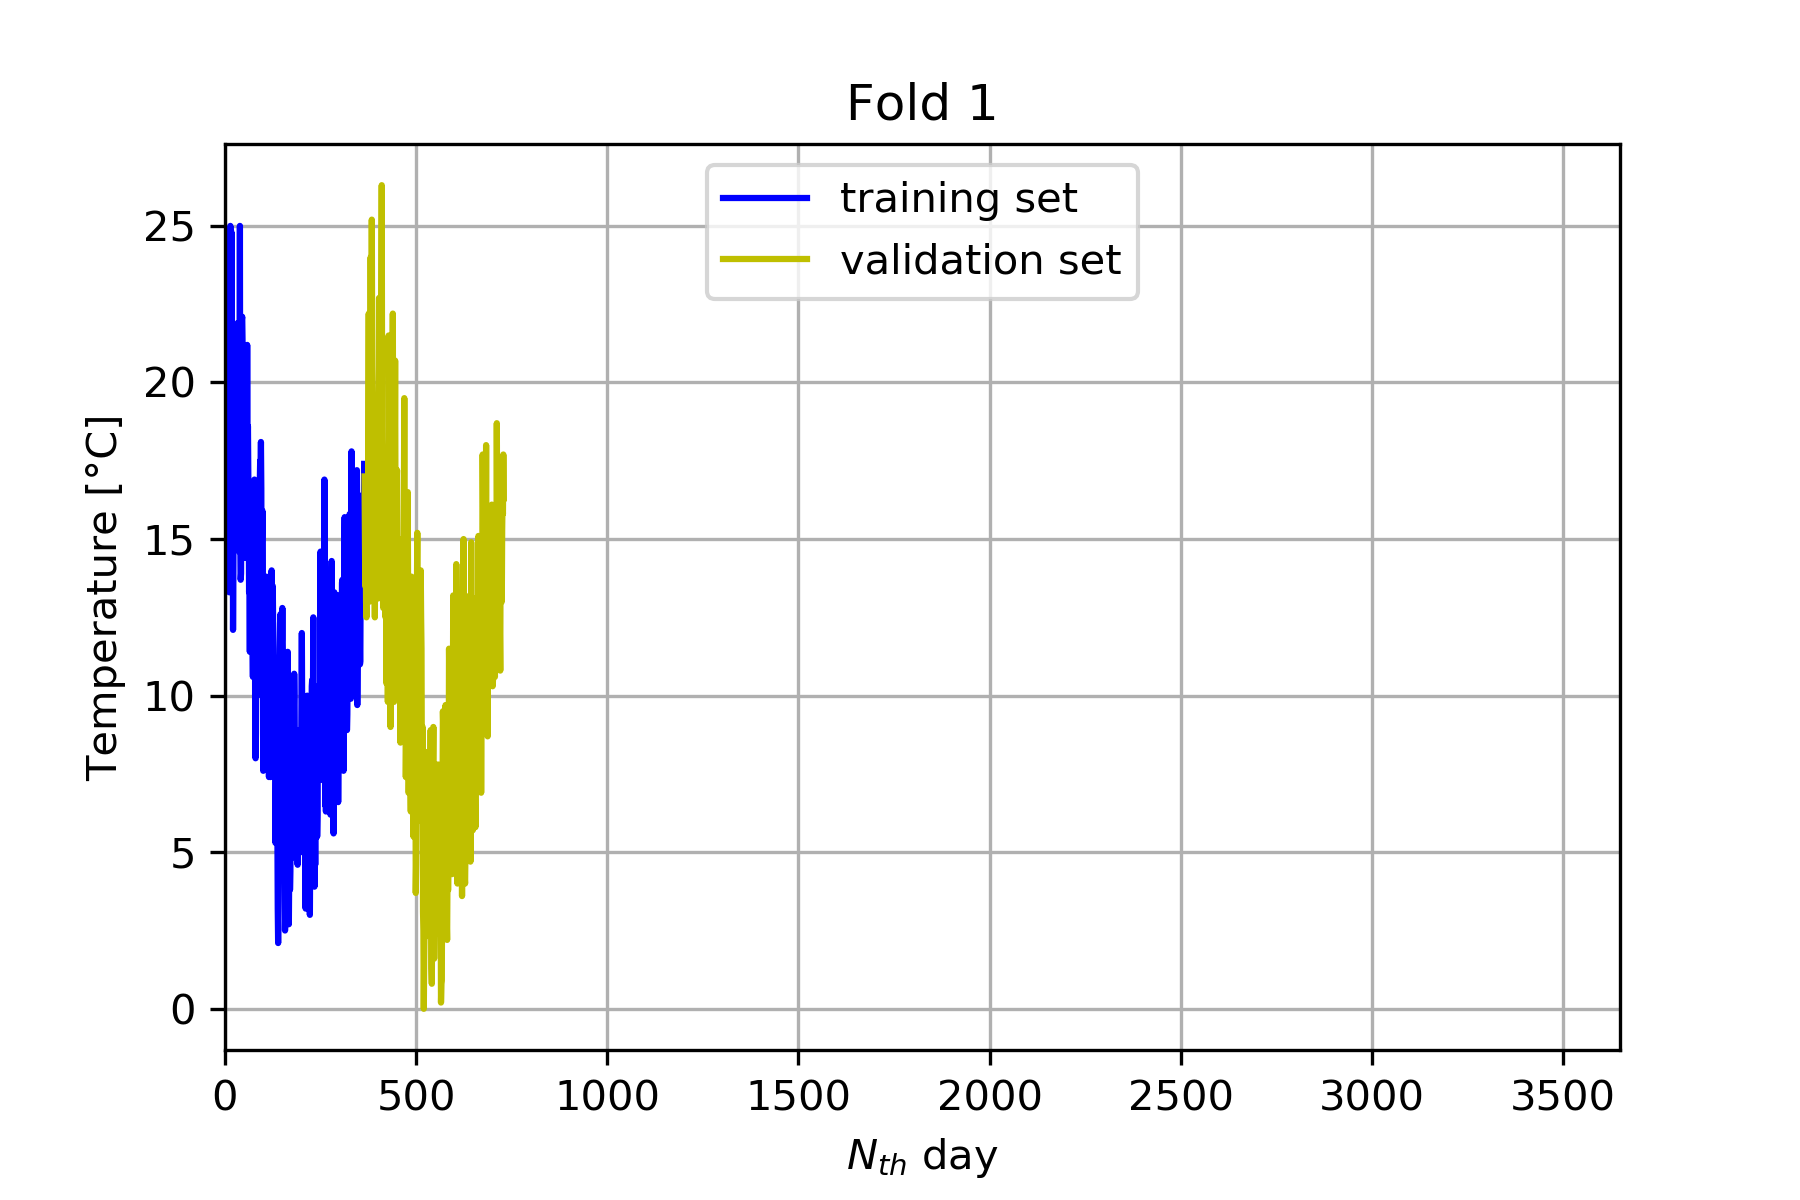
\includegraphics[width=3.85cm]{figure_2_fold_1}
        \caption{Fold 1}
        \label{fig:sub2}
    \end{subfigure}
    \hfill
    % fold 2
    \begin{subfigure}{0.32\textwidth}
        \centering
        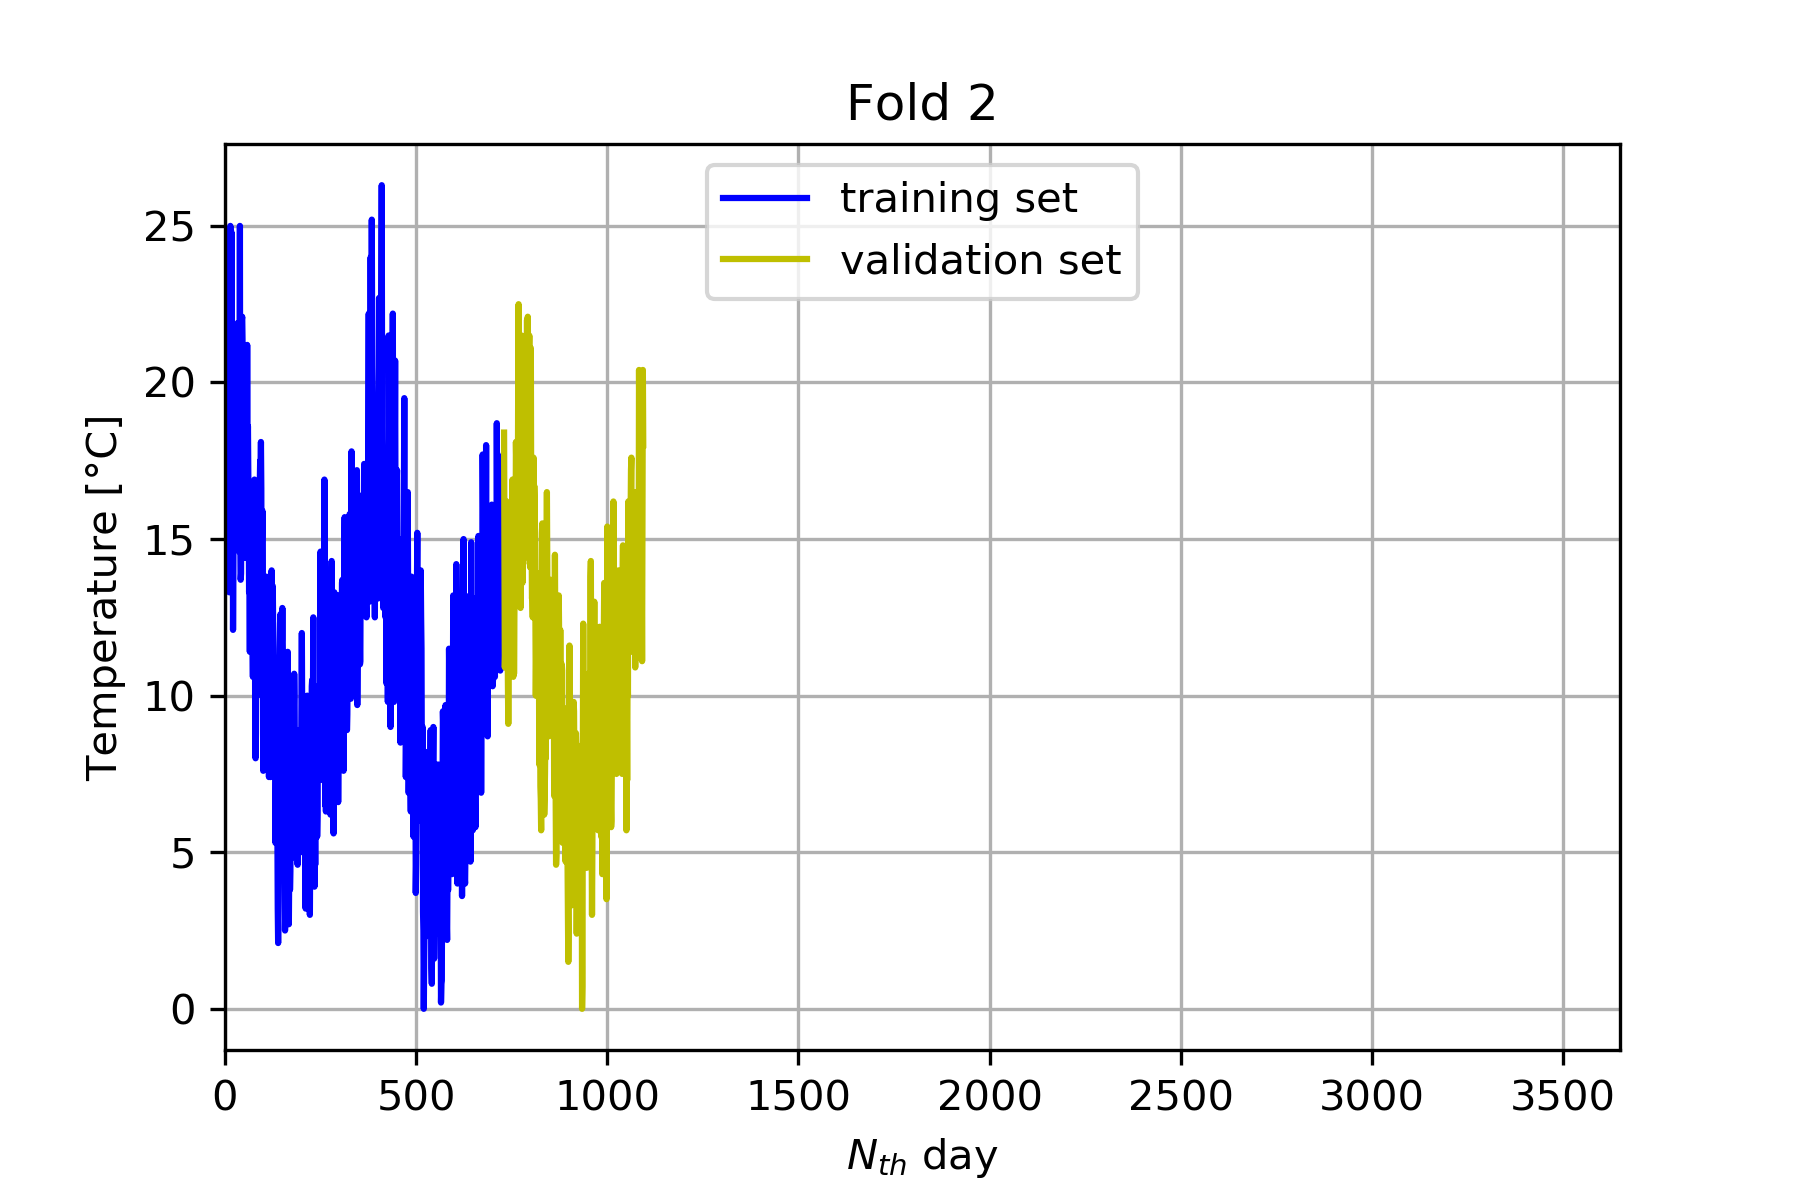
\includegraphics[width=3.85cm]{figure_3_fold_2}
        \caption{Fold 2}
        \label{fig:sub3}
    \end{subfigure}%
    \\
    % fold 3
    \begin{subfigure}{0.32\textwidth}
        \centering
        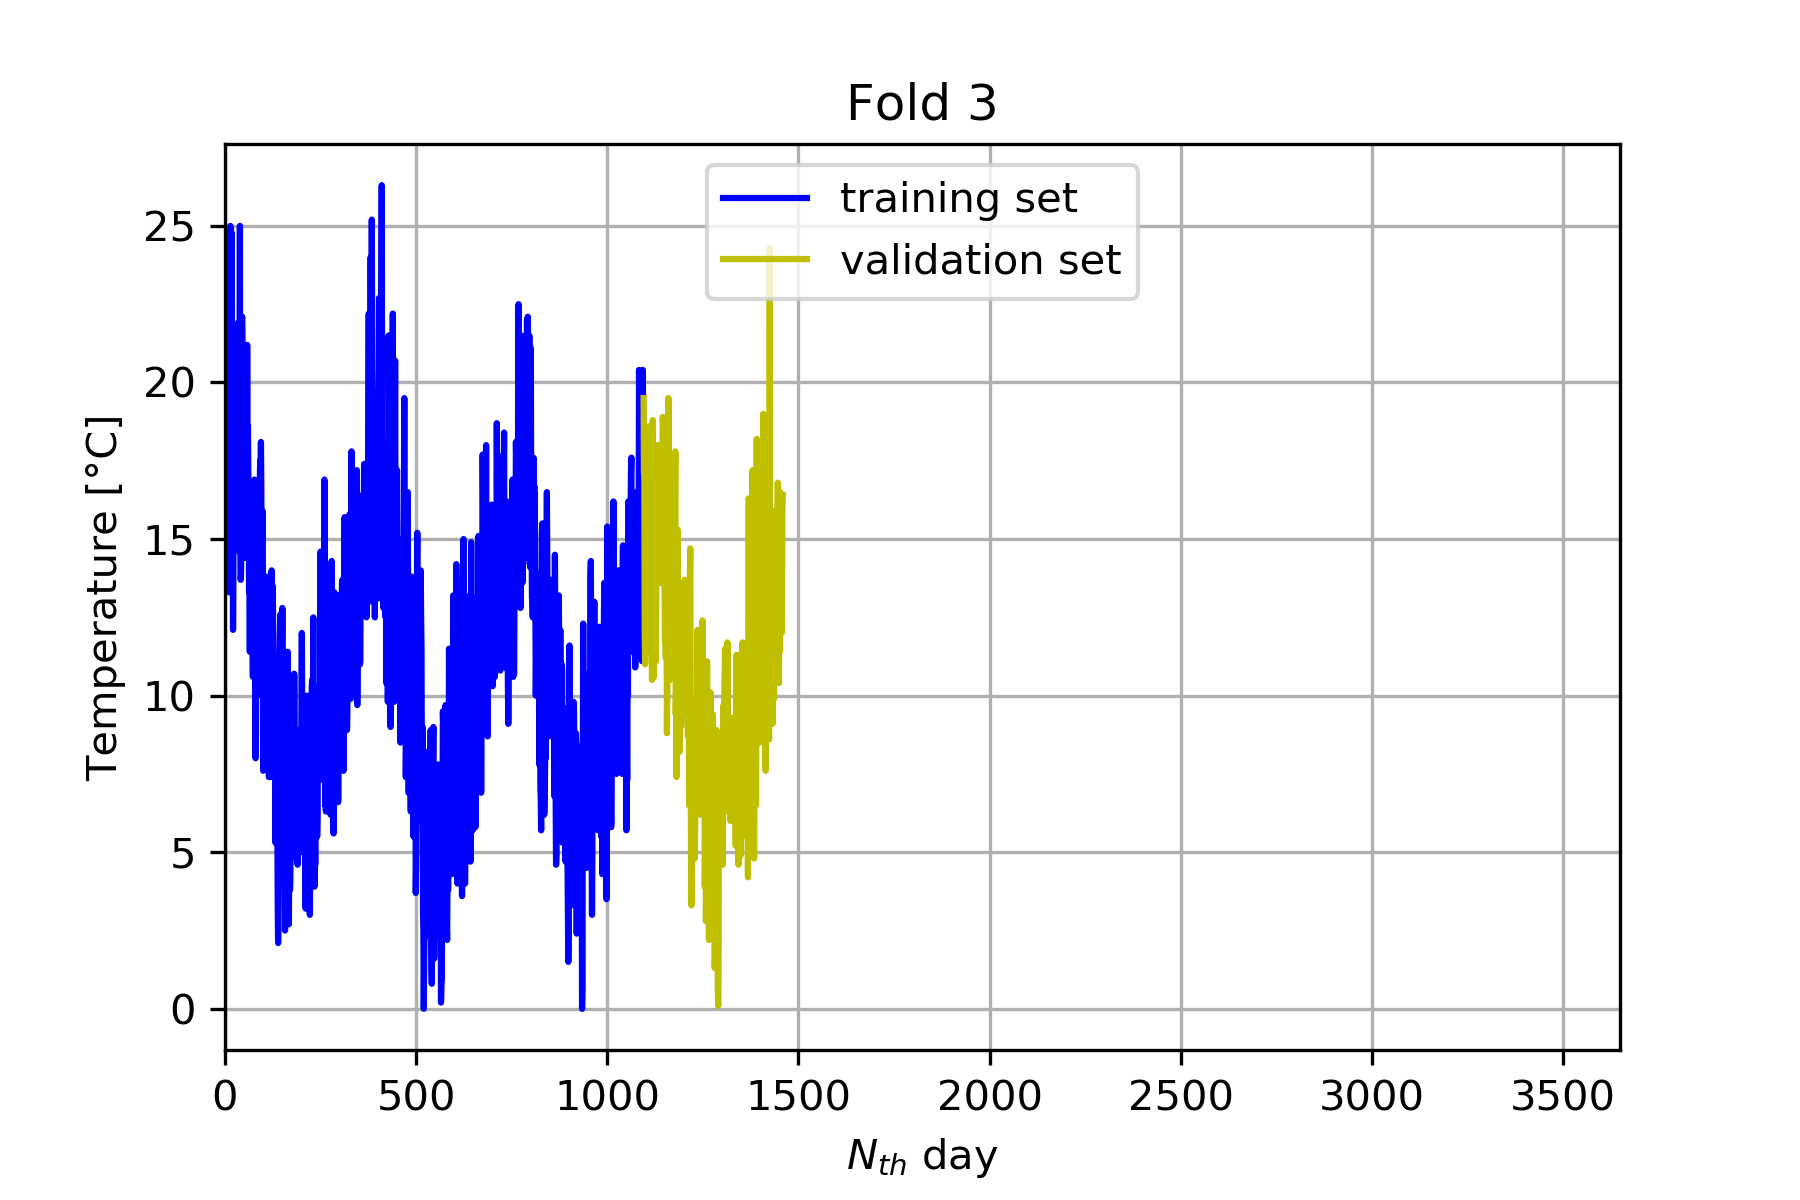
\includegraphics[width=3.85cm]{figure_4_fold_3}
        \caption{Fold 3}
        \label{fig:sub4}
    \end{subfigure}\hfill
    % fold 4
    \begin{subfigure}{0.32\textwidth}
        \centering
        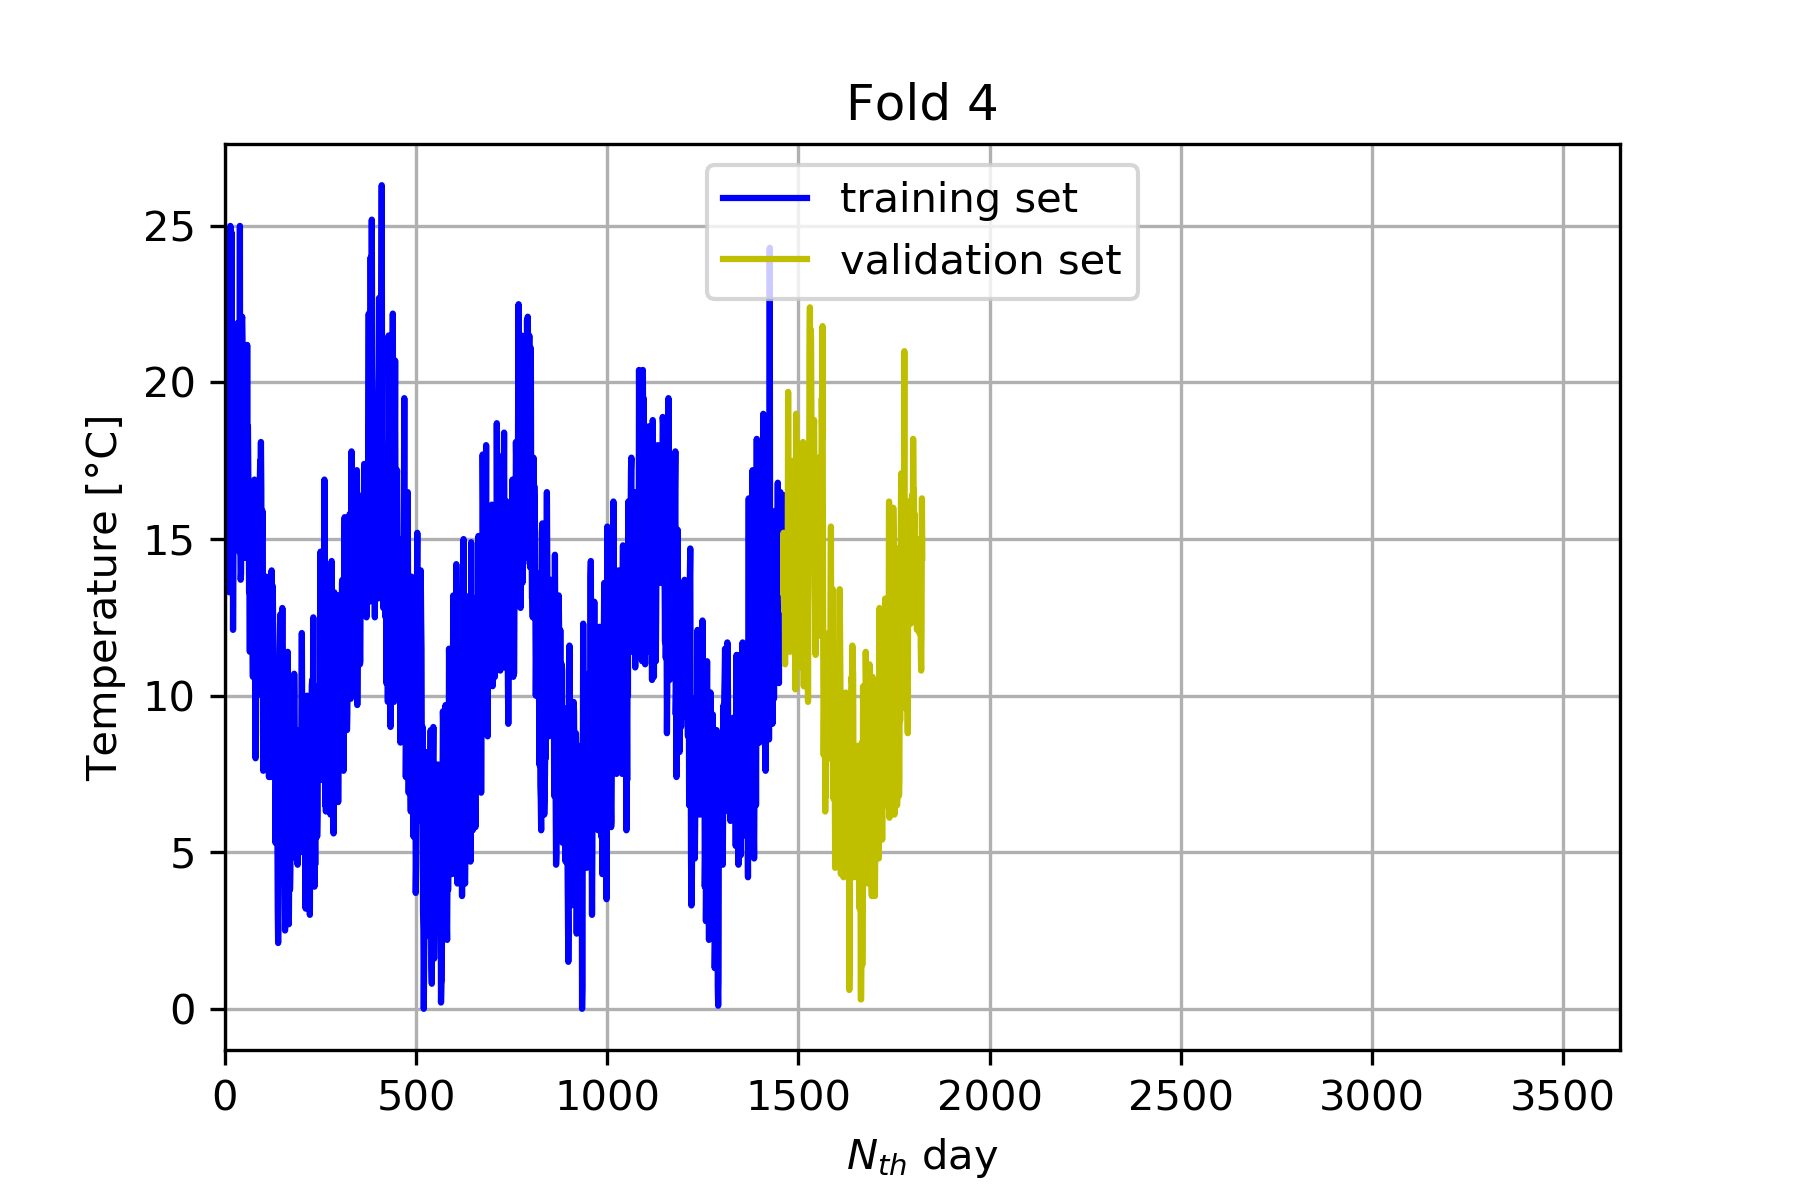
\includegraphics[width=3.85cm]{figure_5_fold_4}
        \caption{Fold 4}
        \label{fig:sub5}
    \end{subfigure}\hfill
    % fold 5
    \begin{subfigure}{0.32\textwidth}
        \centering
        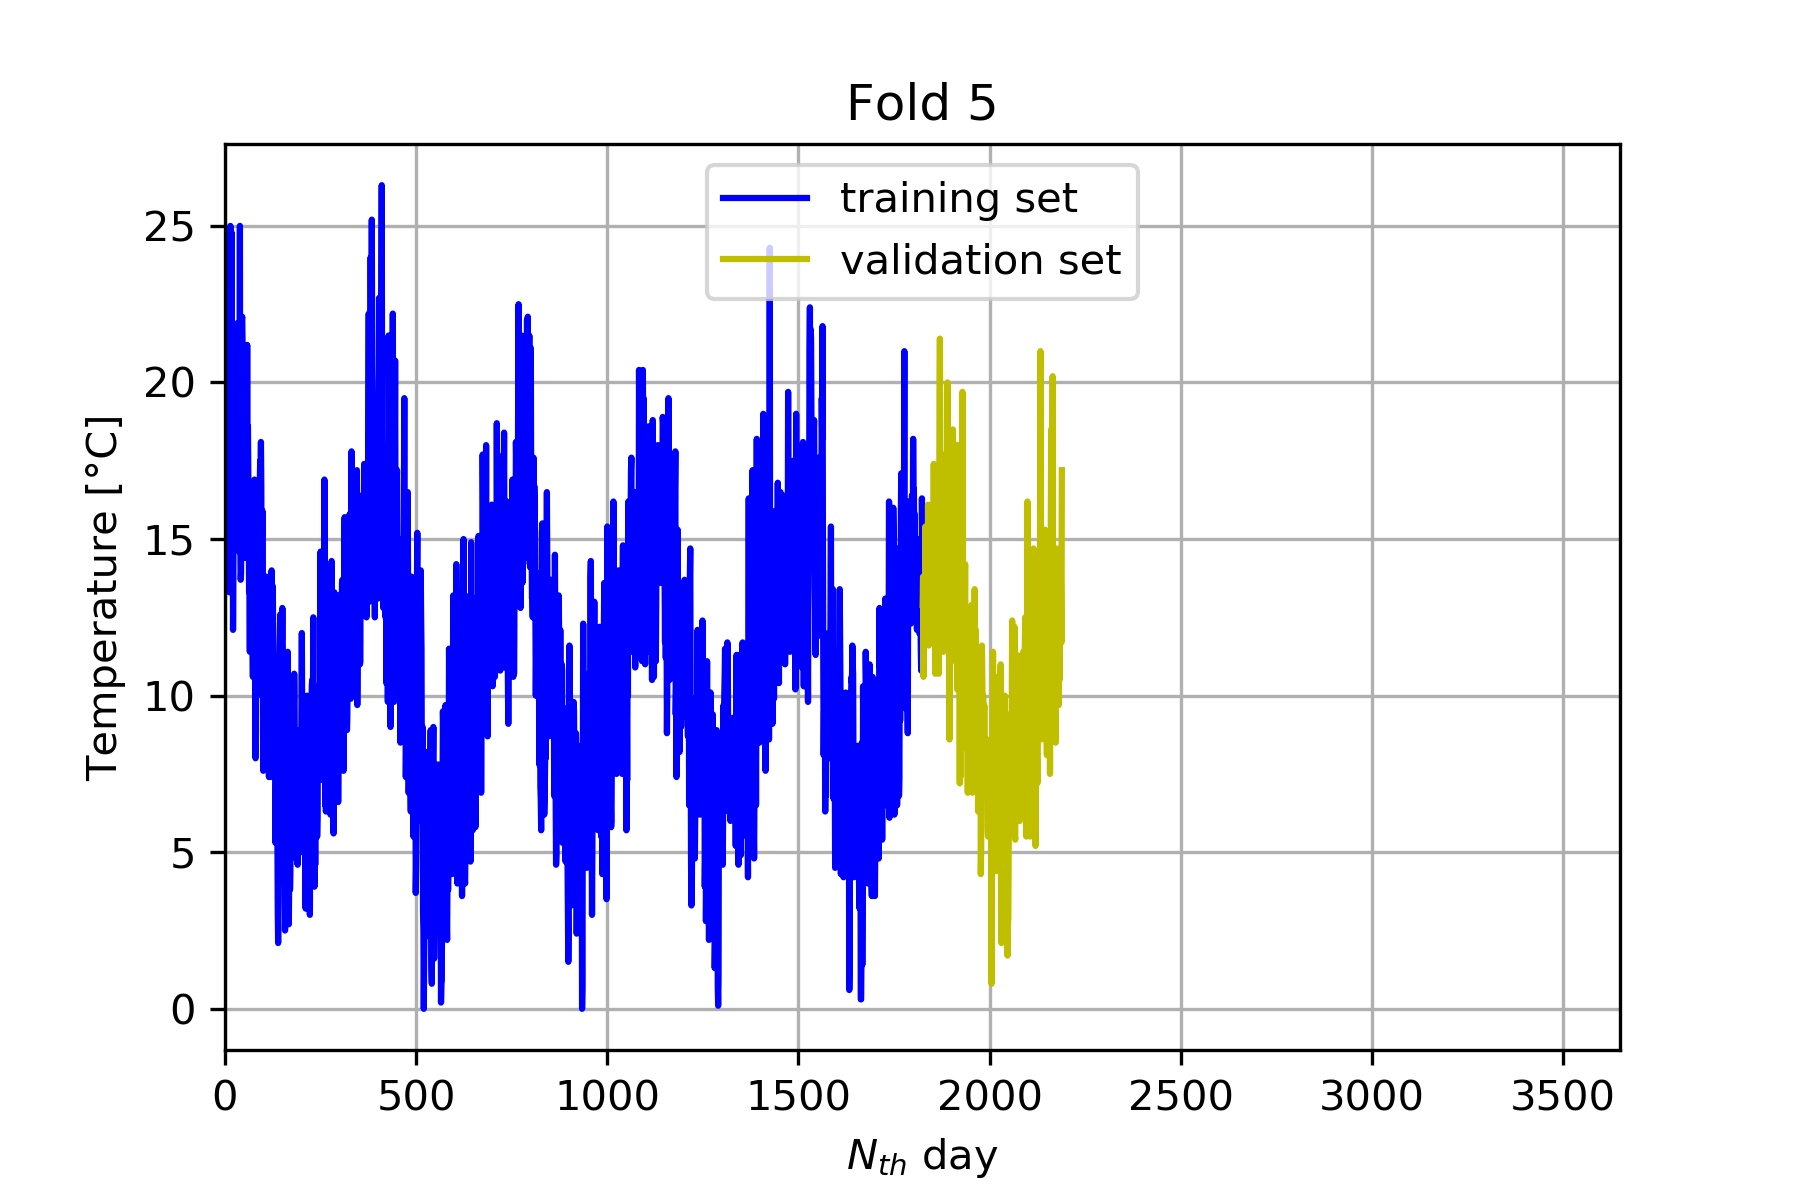
\includegraphics[width=3.85cm]{figure_6_fold_5}
        \caption{Fold 5}
        \label{fig:sub6}
    \end{subfigure}
    \\
    % fold 6
    \begin{subfigure}{0.32\textwidth}
        \centering
        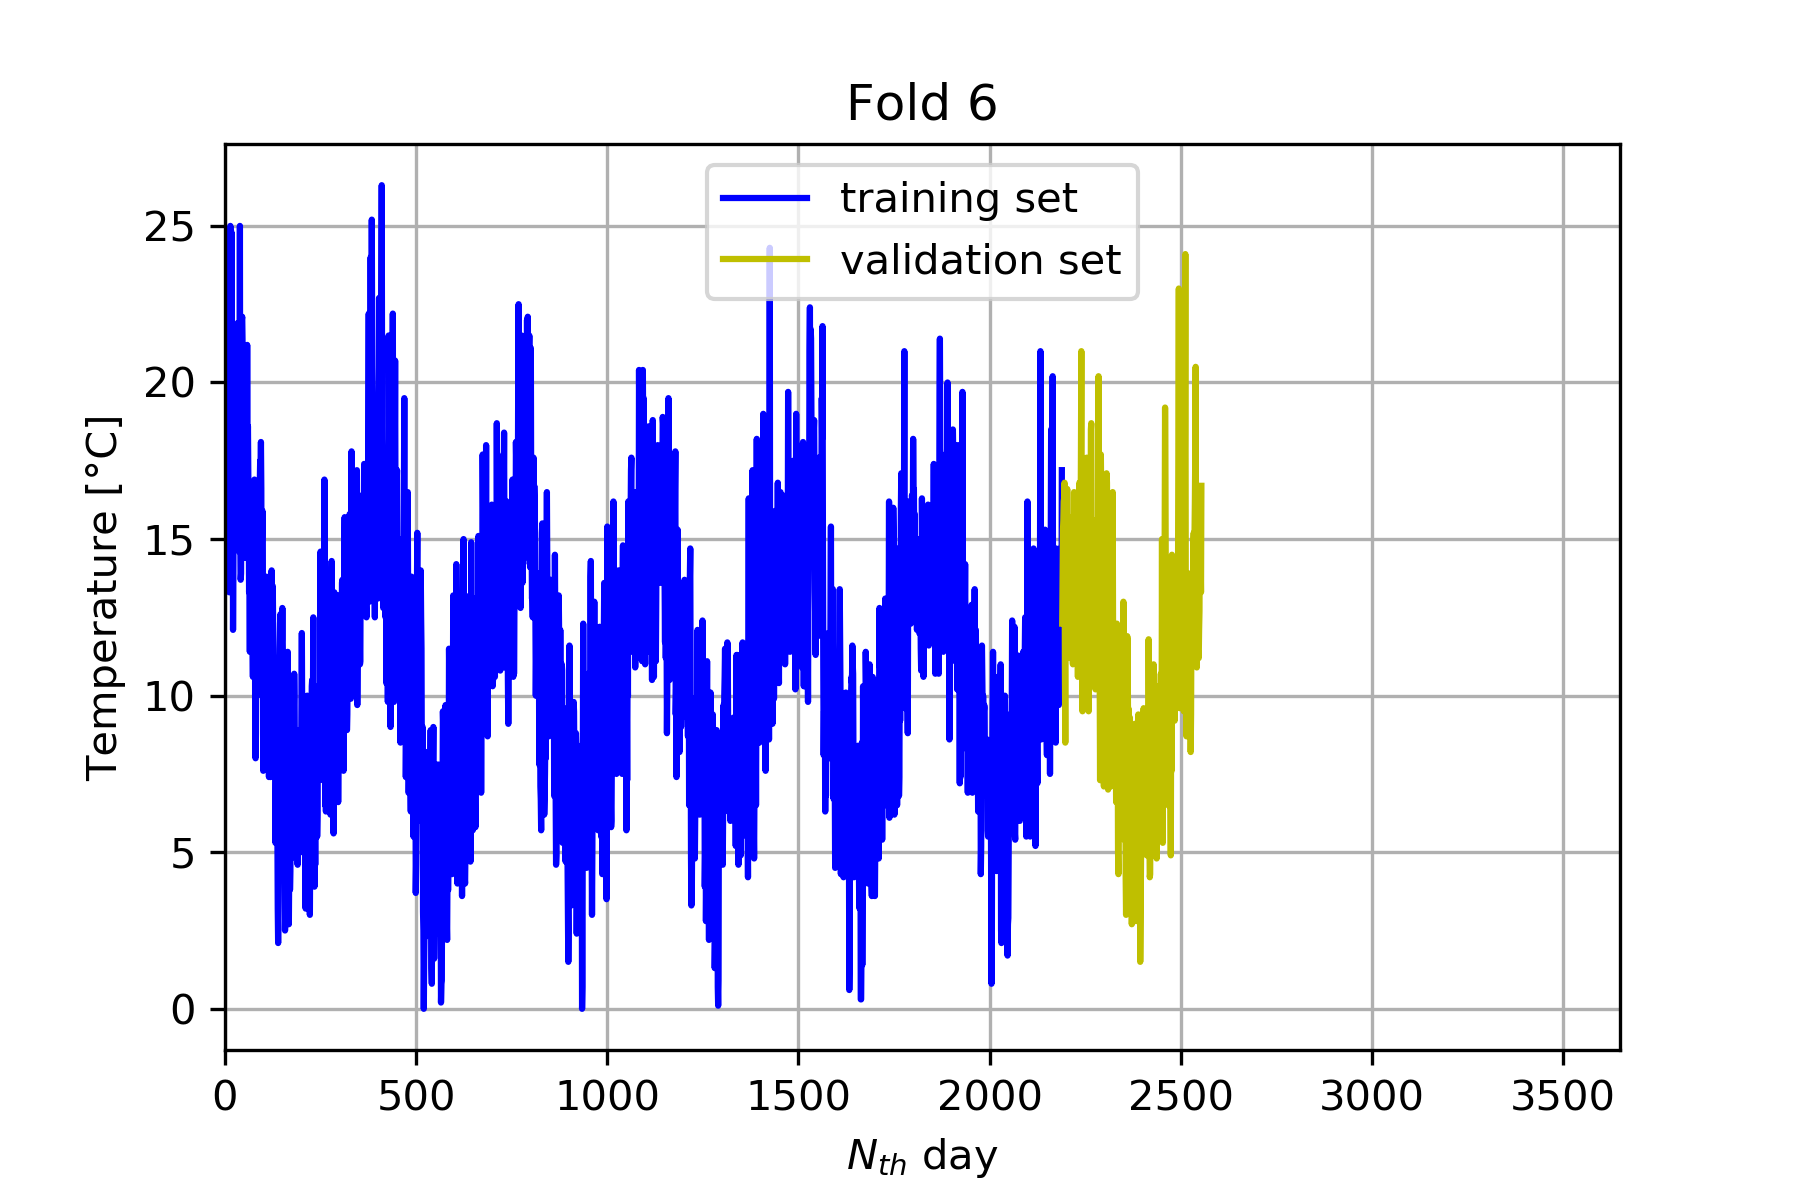
\includegraphics[width=3.85cm]{figure_7_fold_6}
        \caption{Fold 6}
        \label{fig:sub7}
    \end{subfigure}\hfill
    % fold 7
    \begin{subfigure}{0.32\textwidth}
        \centering
        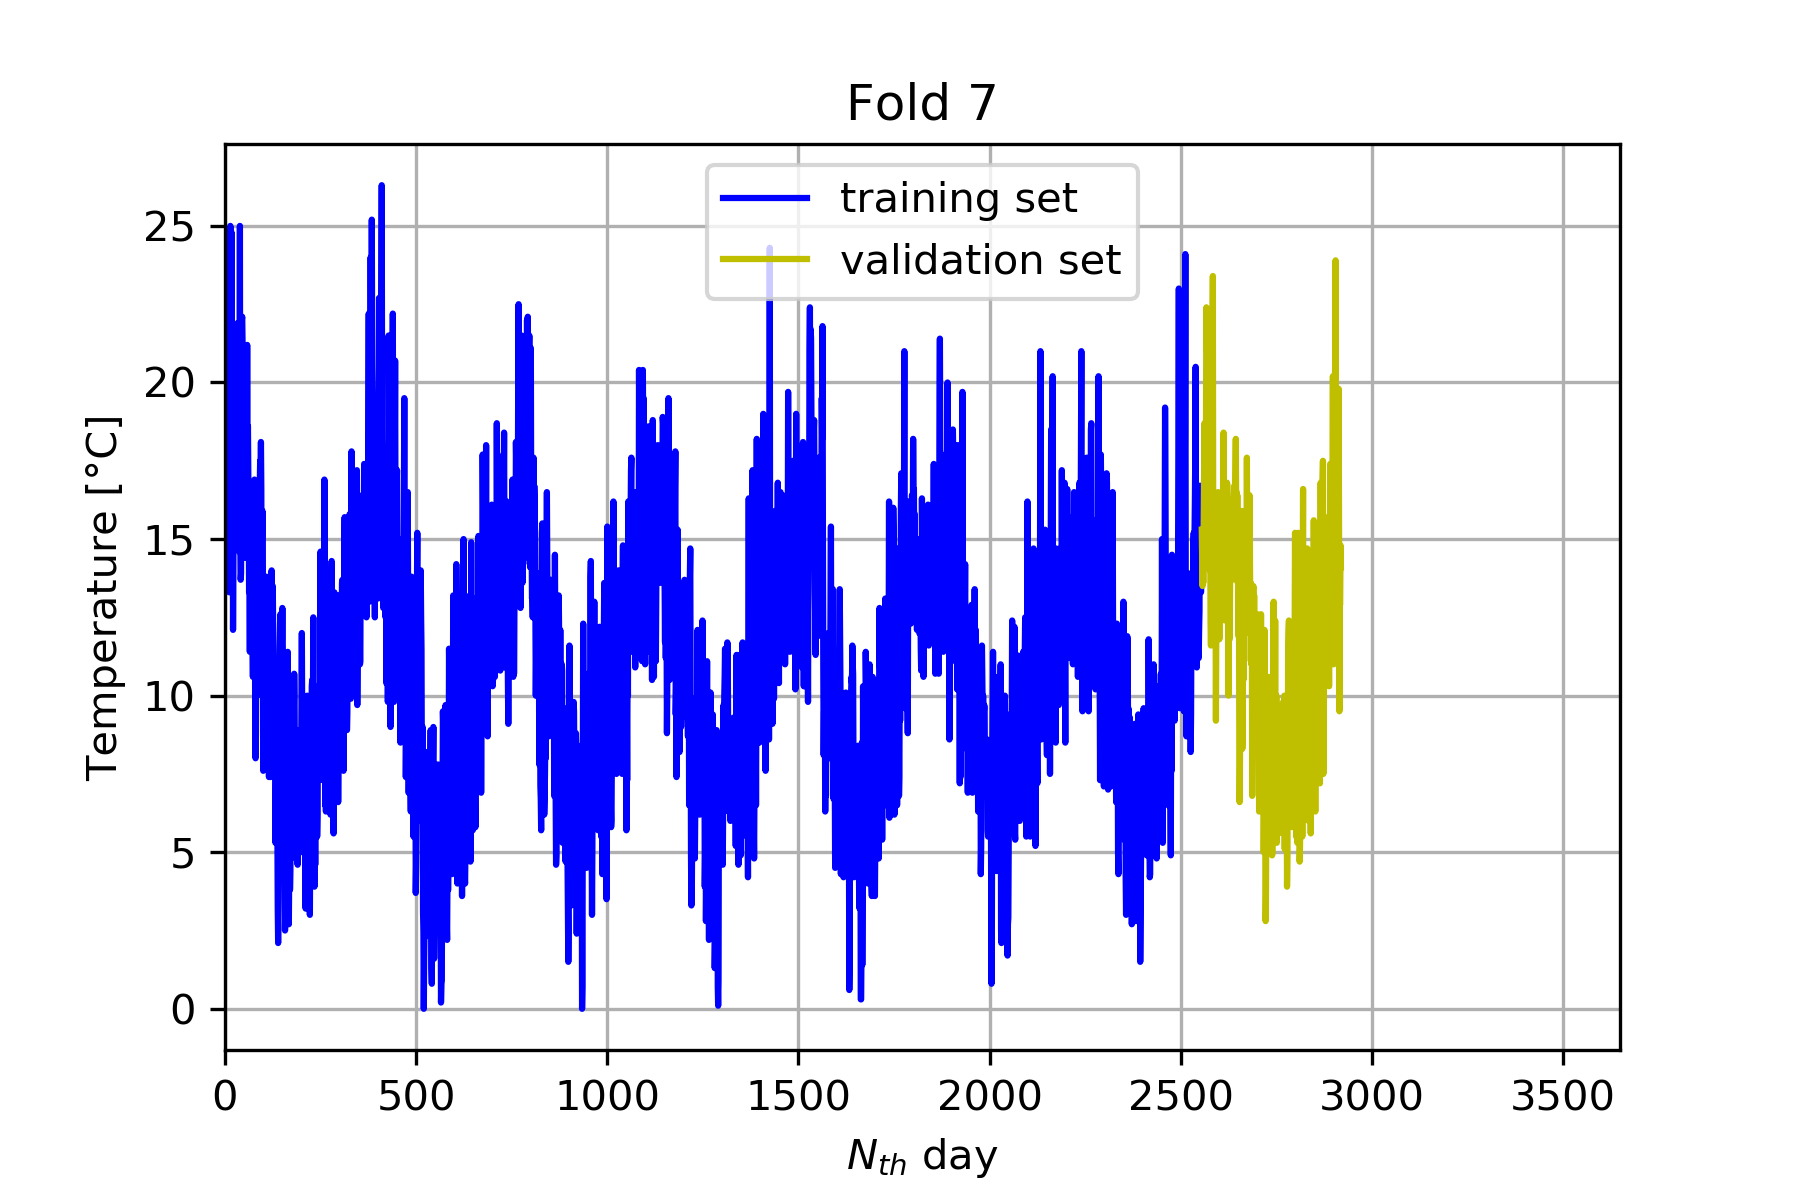
\includegraphics[width=3.85cm]{figure_8_fold_7}
        \caption{Fold 7}
        \label{fig:sub8}
    \end{subfigure}\hfill
    % fold 8
    \begin{subfigure}{0.32\textwidth}
        \centering
        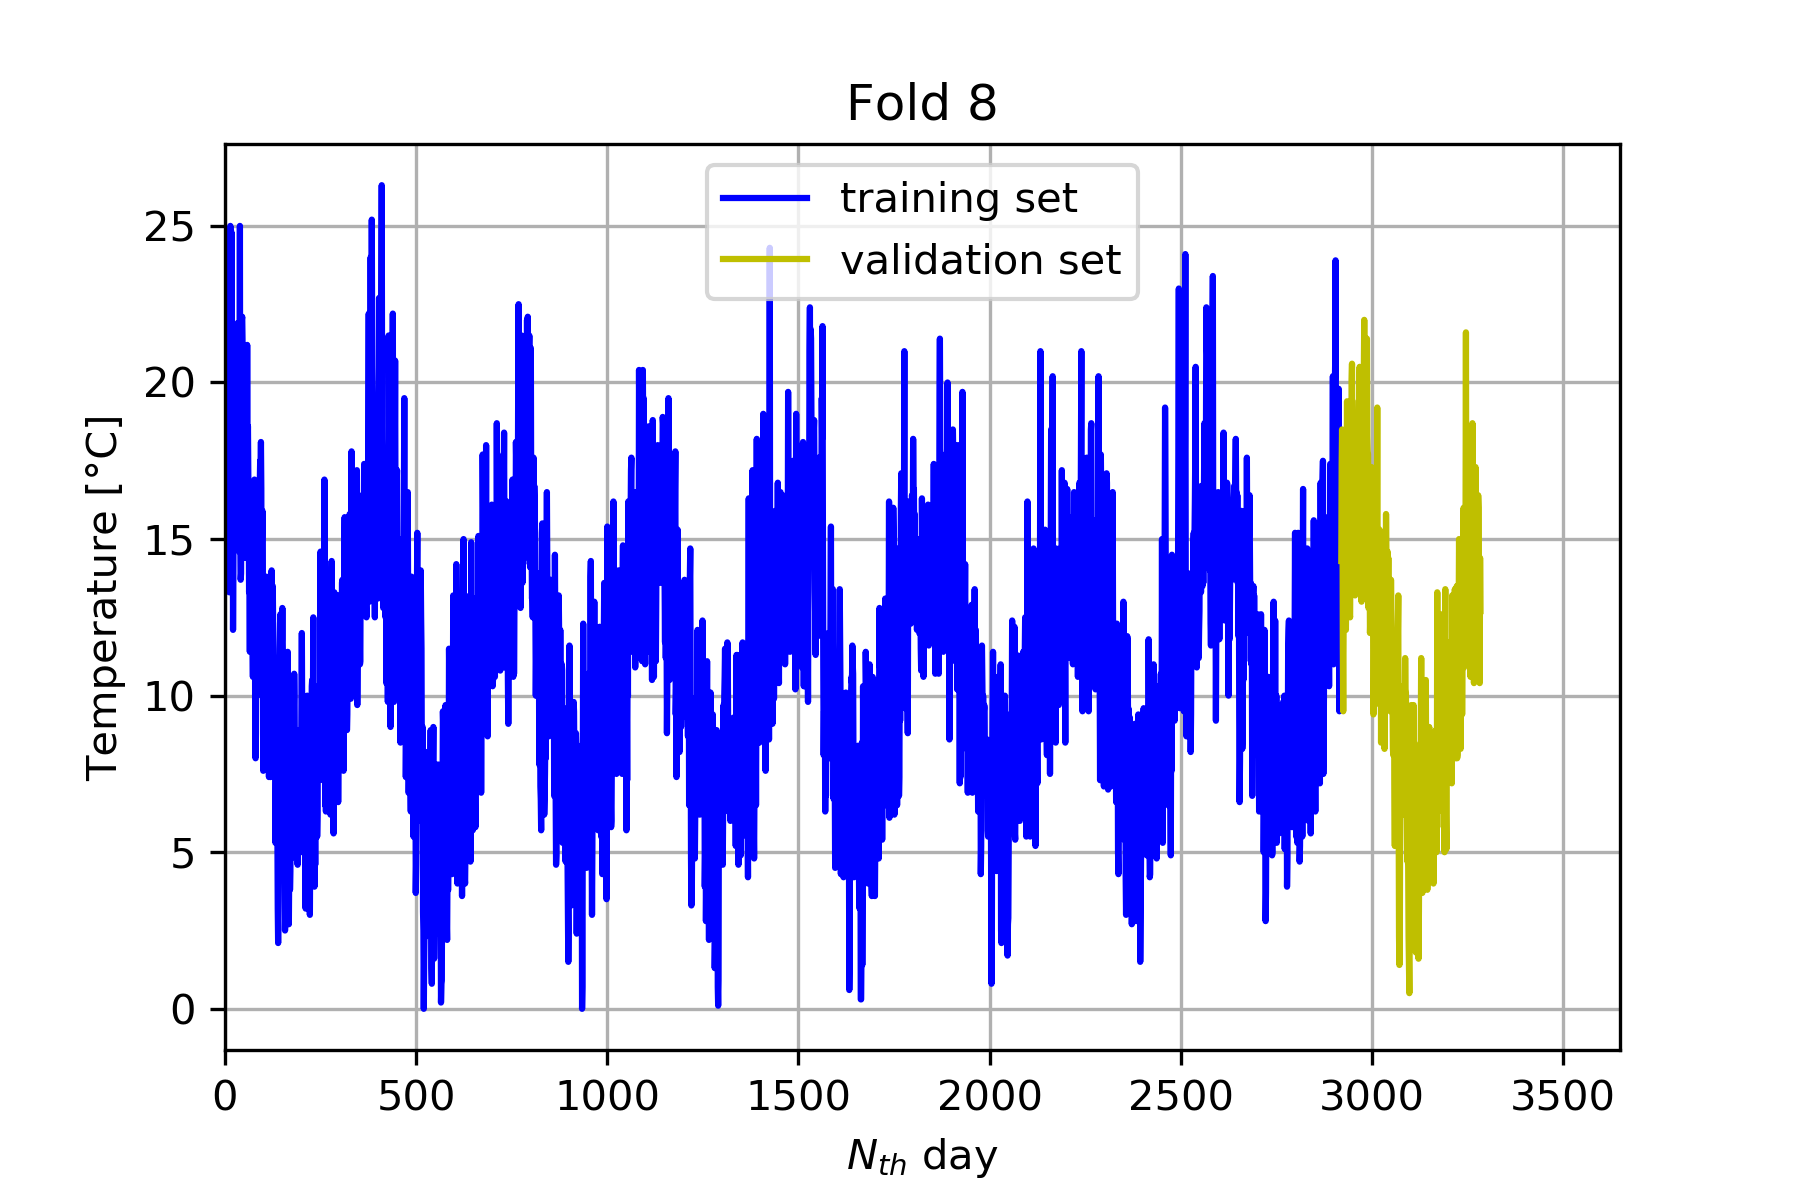
\includegraphics[width=3.85cm]{figure_9_fold_8}
        \caption{Fold 8}
        \label{fig:sub9}
    \end{subfigure}
    % caption and label
    \caption{Folds used in cross-validation}
    \label{fig:pre-ex1-kfold}
\end{figure}

\paragraph{The goal of using this method of cross-validation is to find the best value for the hyperparameter K, the number of previous days used as input for the model.\\After choosing the hyperparameter, we no more use the folds division. Instead, all data before used for training and validation is now used only for training. This can be considered as the last training of the model and the one which will return the weights desired in this problem of linear regression. This can be seen in figure \ref{fig:pre-ex1-10}.}

\begin{figure}[H]
    \centering
    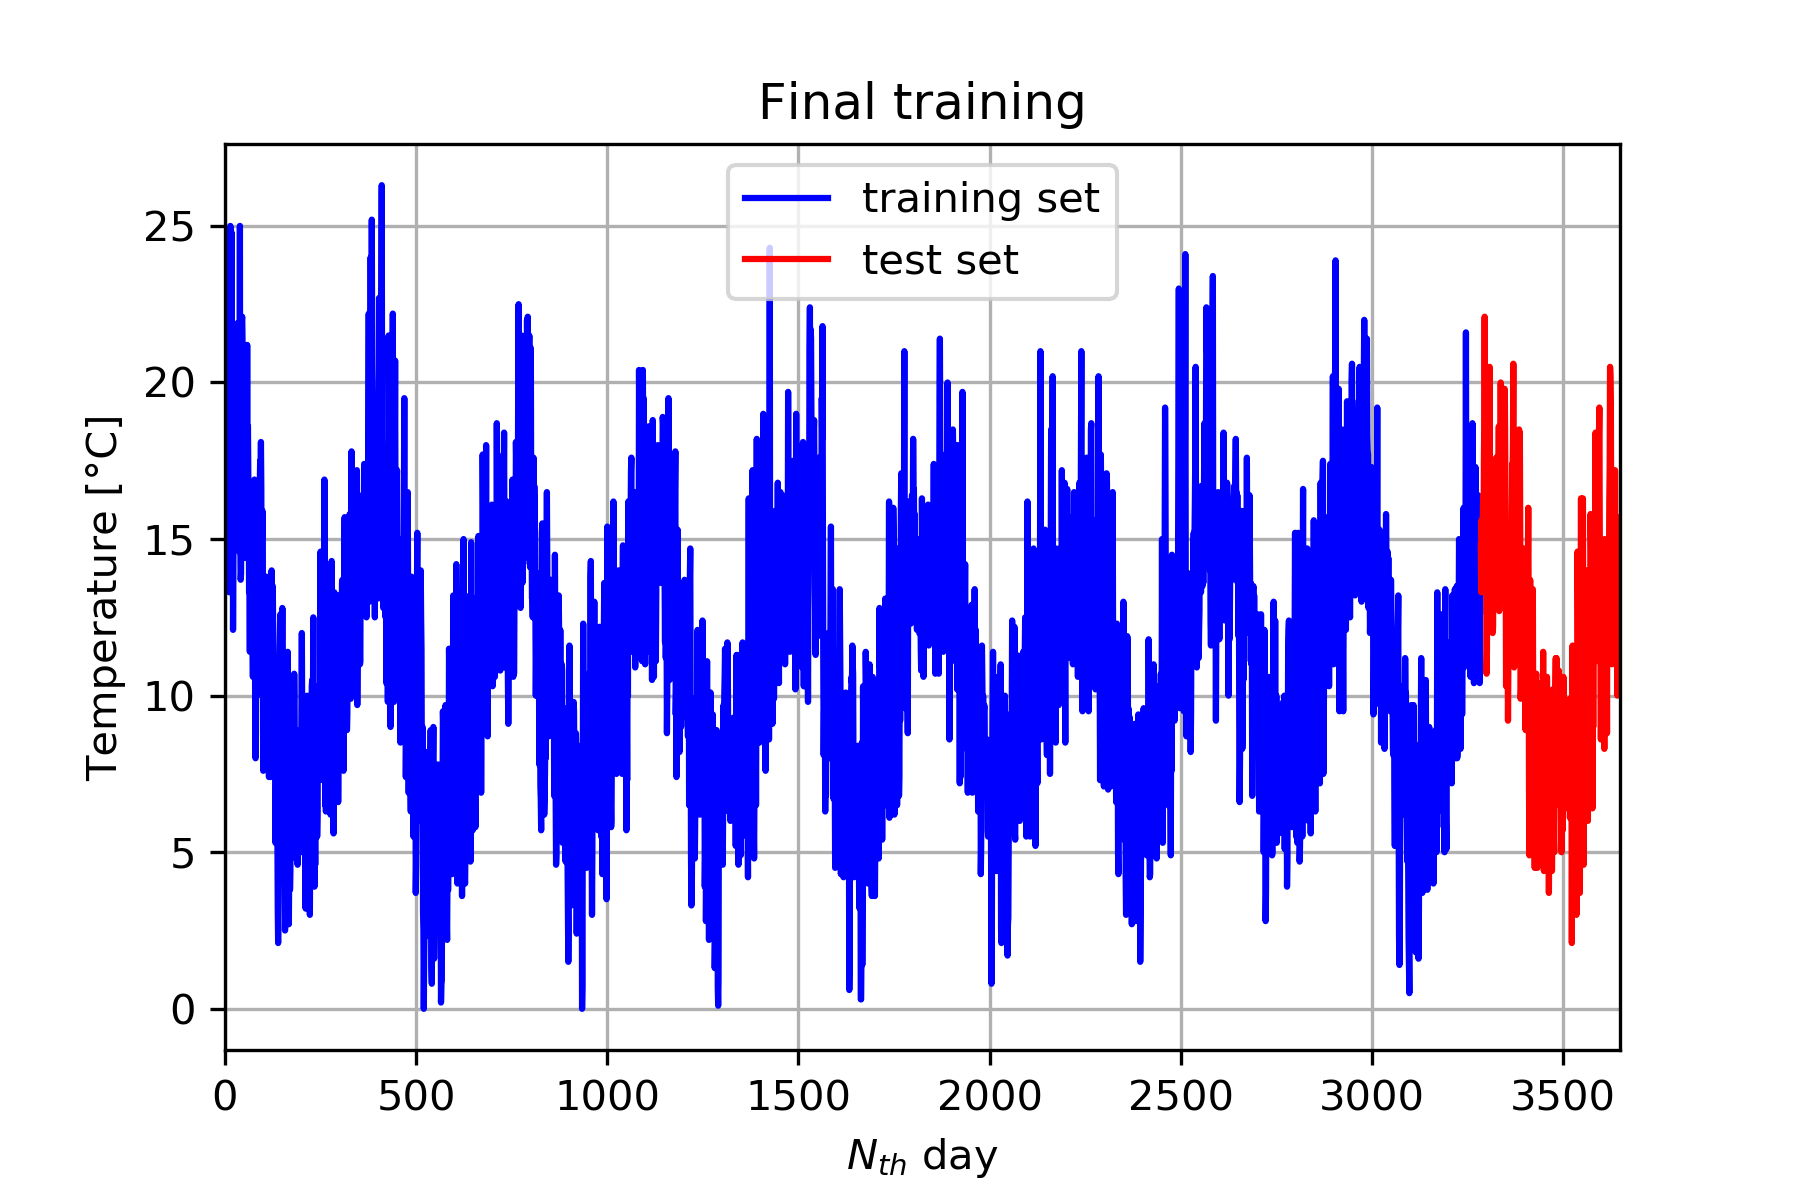
\includegraphics[width=12cm]{figure_10_final_training}
    \caption{}
    \label{fig:pre-ex1-10}
\end{figure}

%==============================
\subsubsection{a) Progression of the RMSE measured in validation set in function of hyperparameter K (from 1 to 31):}
%==============================

\paragraph{The model was trained for values of the hyperparameter K from 1 to 31 days. The progression of the root mean squared error (RMSE) measured in the validation set can be seen in figure \ref{fig:ex1-1}.}

\begin{figure}[H]
    \centering
    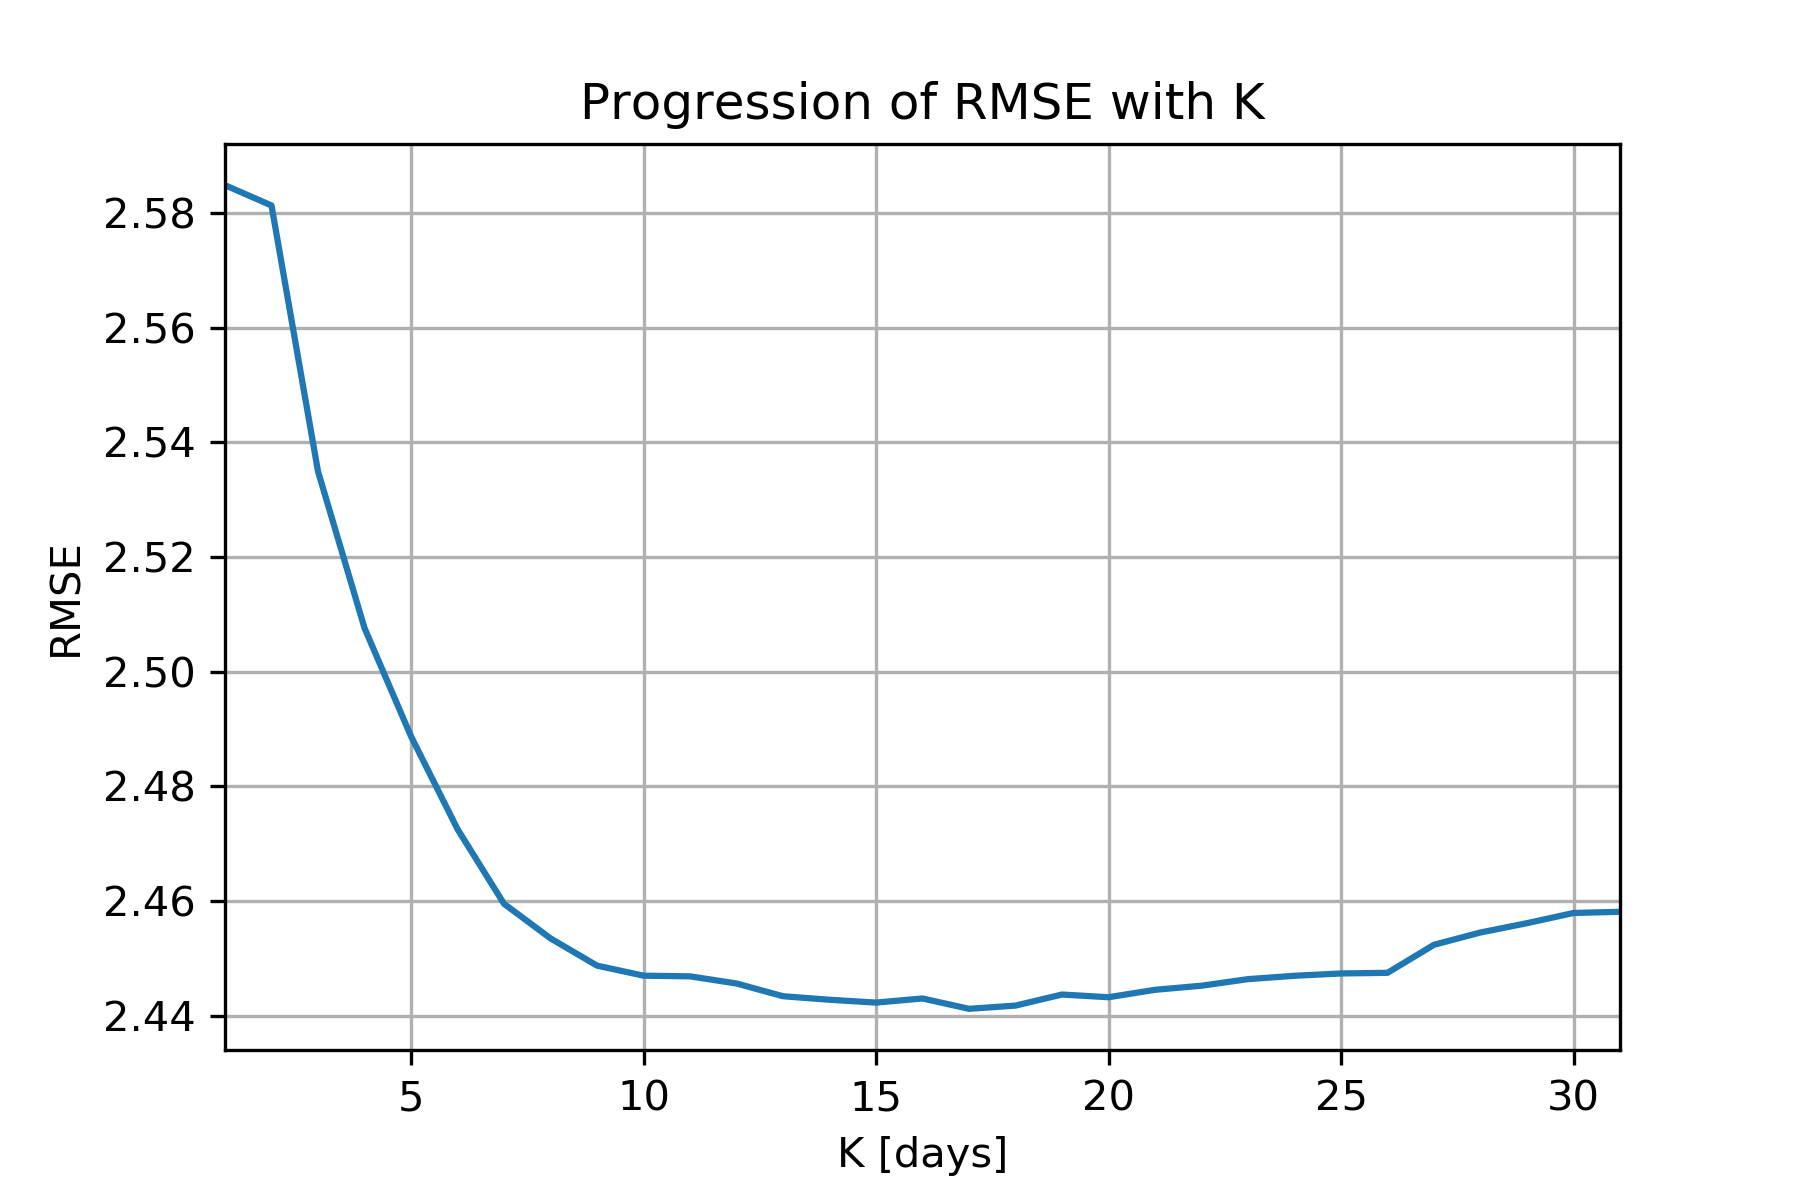
\includegraphics[width=12cm]{figure_1_rmse_with_k}
    \caption{}
    \label{fig:ex1-1}
\end{figure}

\paragraph{We can see that the error starts with values bigger than 2.5 degrees Celsius and decreases as K increases. After K equal to 20 days, we can see that the error only increases, possibly indicating an overfitting.\\Figure \ref{fig:ex1-2} shows a zoom of the previous curve for values of K from 10 to 24. With this zoomed curve, we can see that the value of K that gives the lowest error is 16.}

\begin{figure}[H]
    \centering
    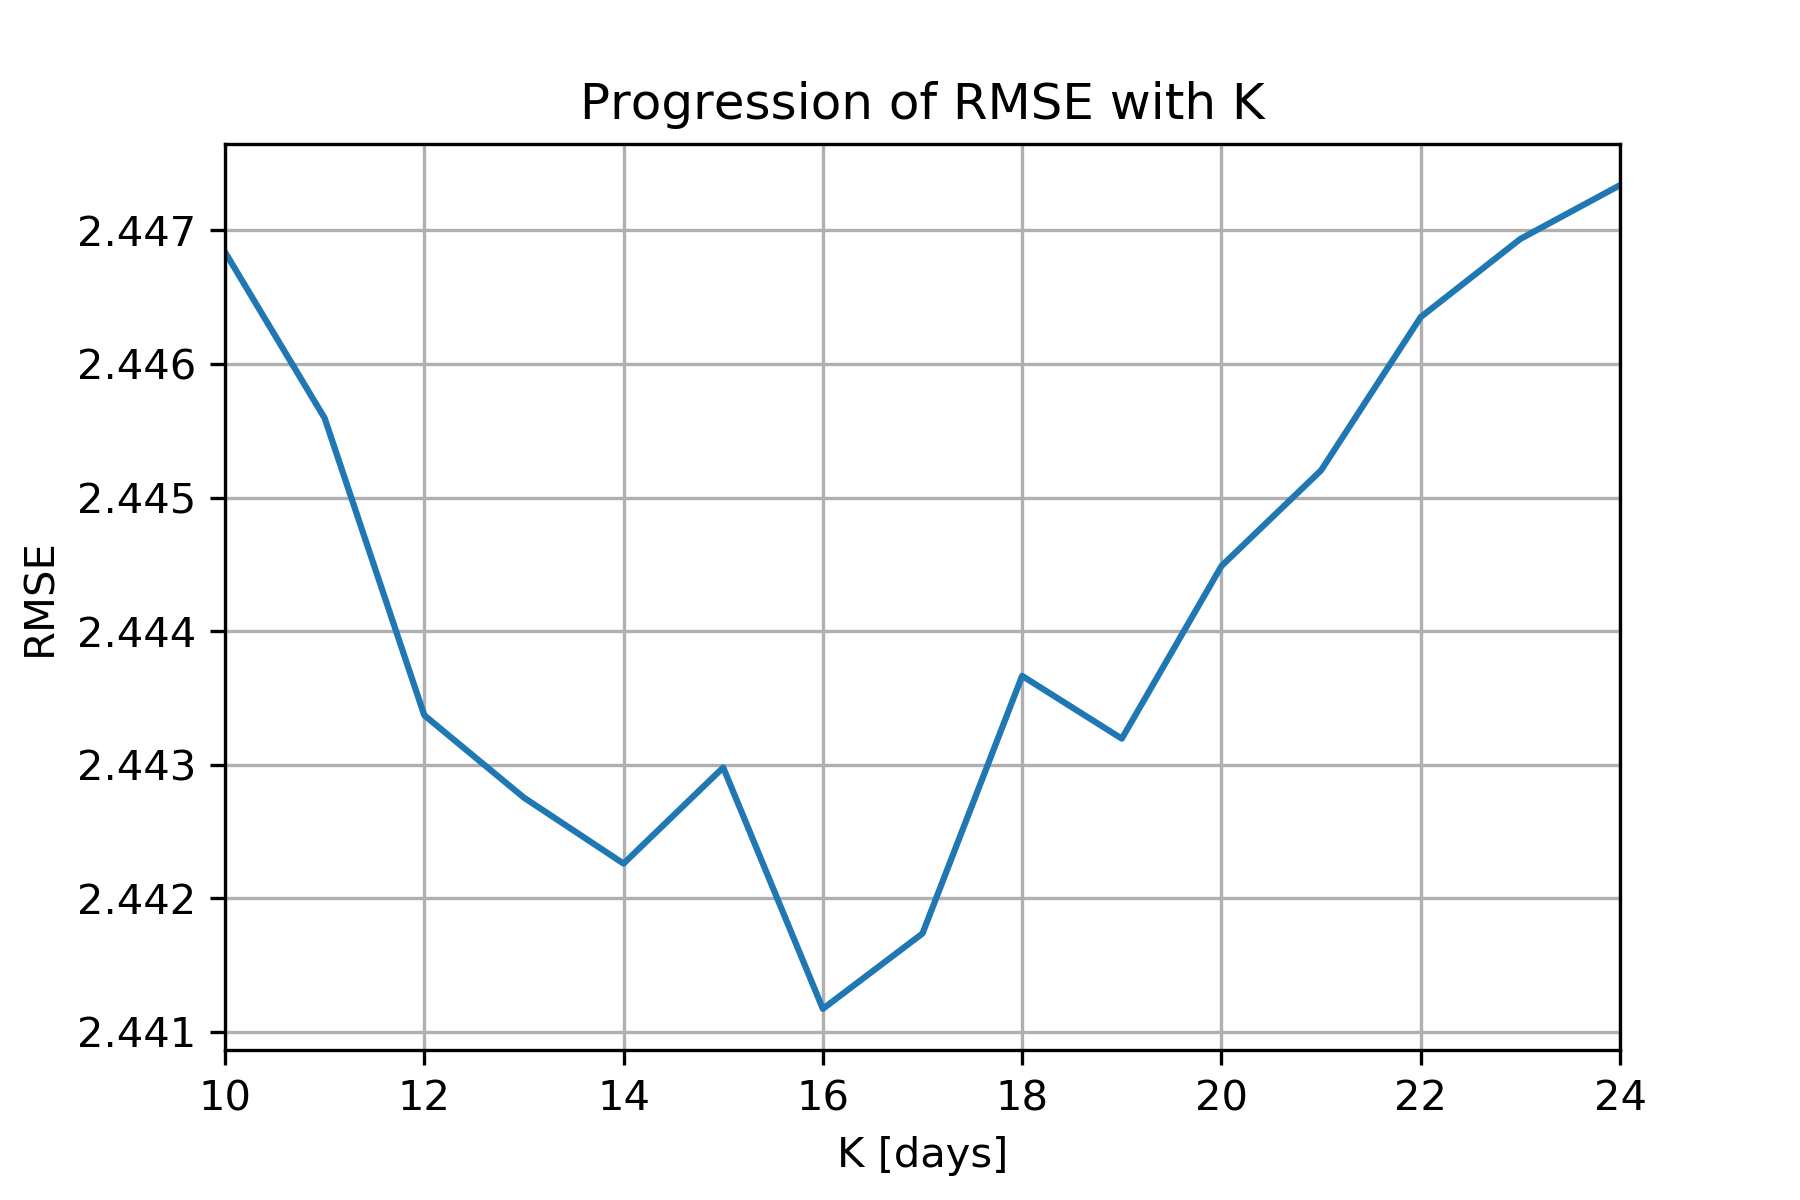
\includegraphics[width=12cm]{figure_2_rmse_with_k_zoom}
    \caption{}
    \label{fig:ex1-2}
\end{figure}

%==============================
\subsubsection{b) Plot of predicted and real temperatures of test set}
%==============================

\paragraph{After finding the optimum K using the k-fold cross-validation, we trained the model considering all data. With the value of the weights, we can compute the predicted minimum temperature for the test set (year 1990) and compare with the real temperatures measured. This plot can be seen in figure \ref{fig:ex1-3}.}

\begin{figure}[H]
    \centering
    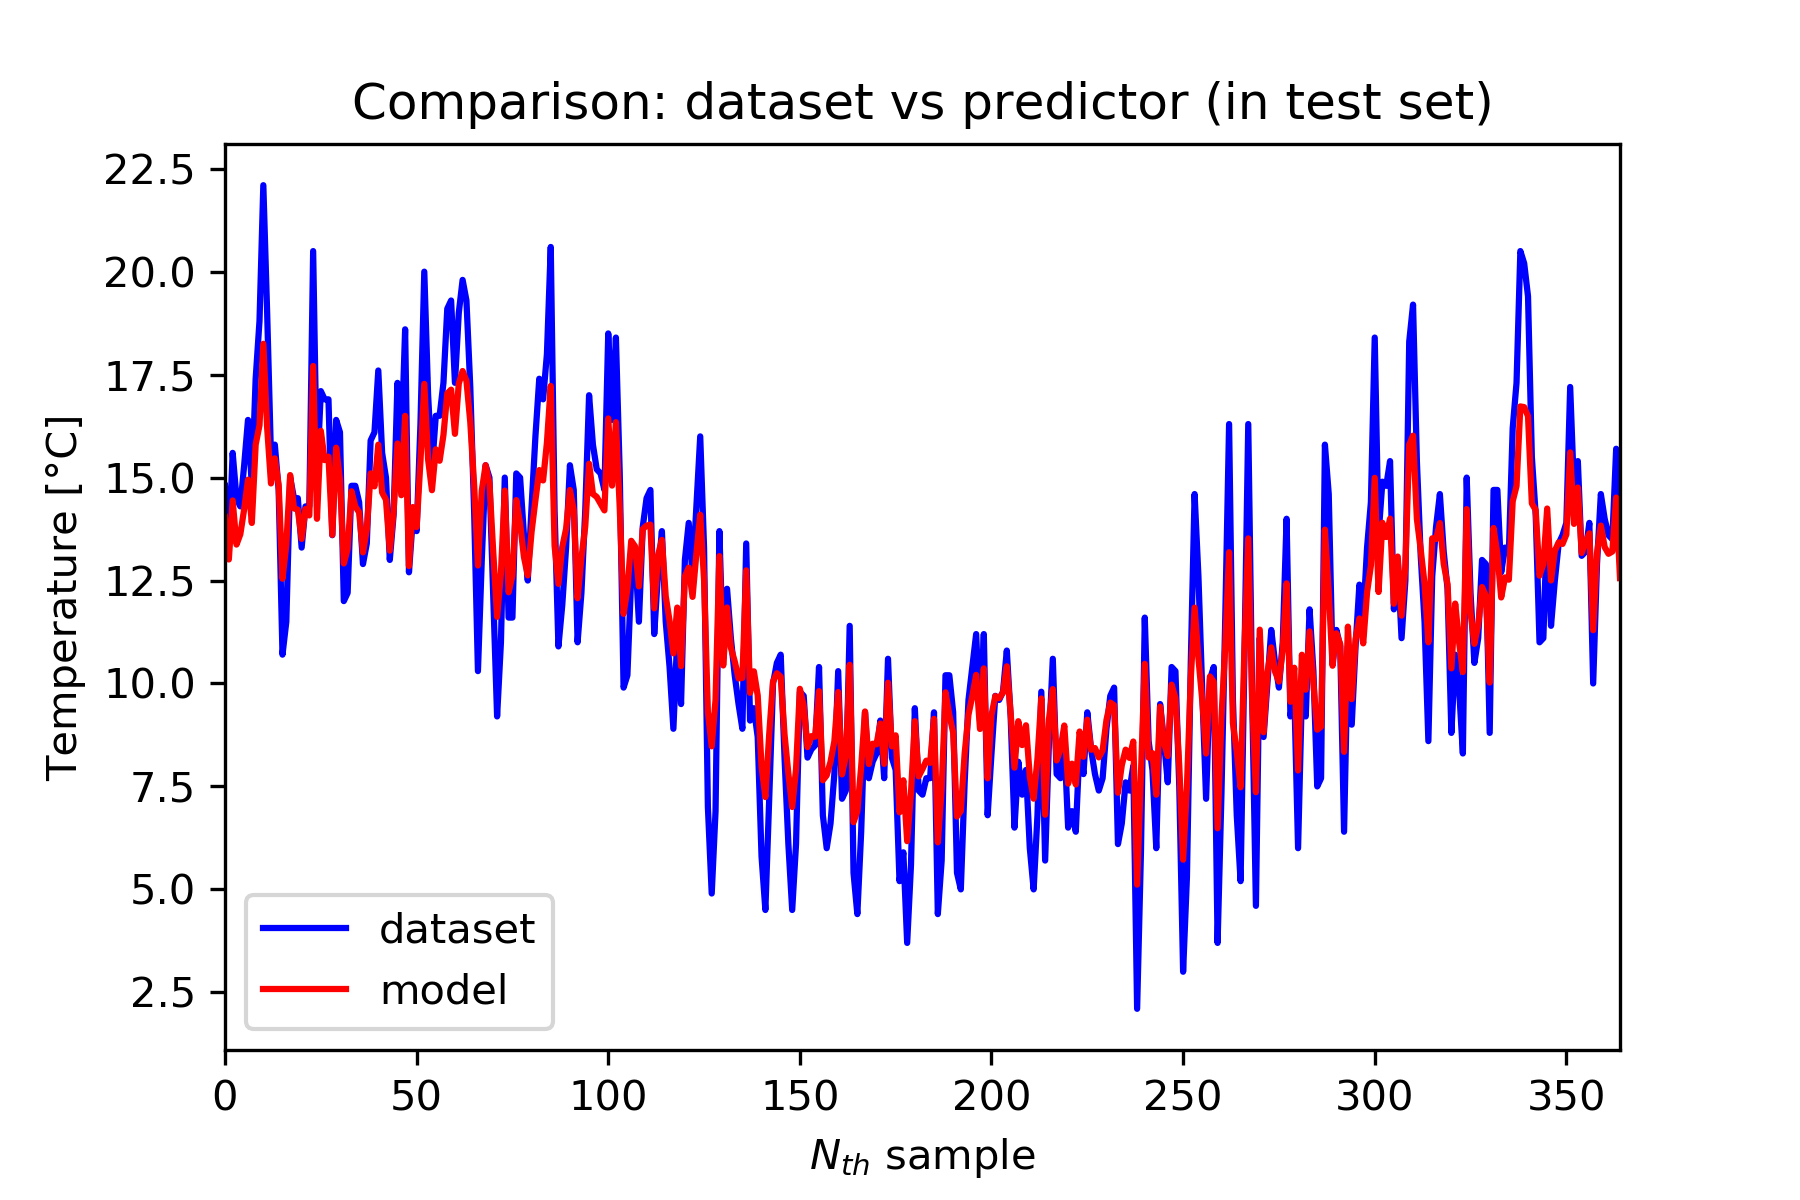
\includegraphics[width=12cm]{figure_3_predictor}
    \caption{}
    \label{fig:ex1-3}
\end{figure}

\paragraph{After calculating the predicted values for all the inputs corresponding to the year 1990, we can calculate the overall RMSE between the predicted values and the real ones. The error measured with this model is 2.279 degrees Celsius.}

%=======================================
\subsection{Exercise 2}
%=======================================

\paragraph{In this exercise, a non-linear transformation applied to the input data is explored in order to try to improve the temperature prediction. The non-linearity suggested is to apply the hyperbolic tangent to the input data. The function of the hyperbolic tangent for values from -5 to 5 can be seen in the figure \ref{fig:pre-ex2-0}.}

\begin{figure}[H]
    \centering
    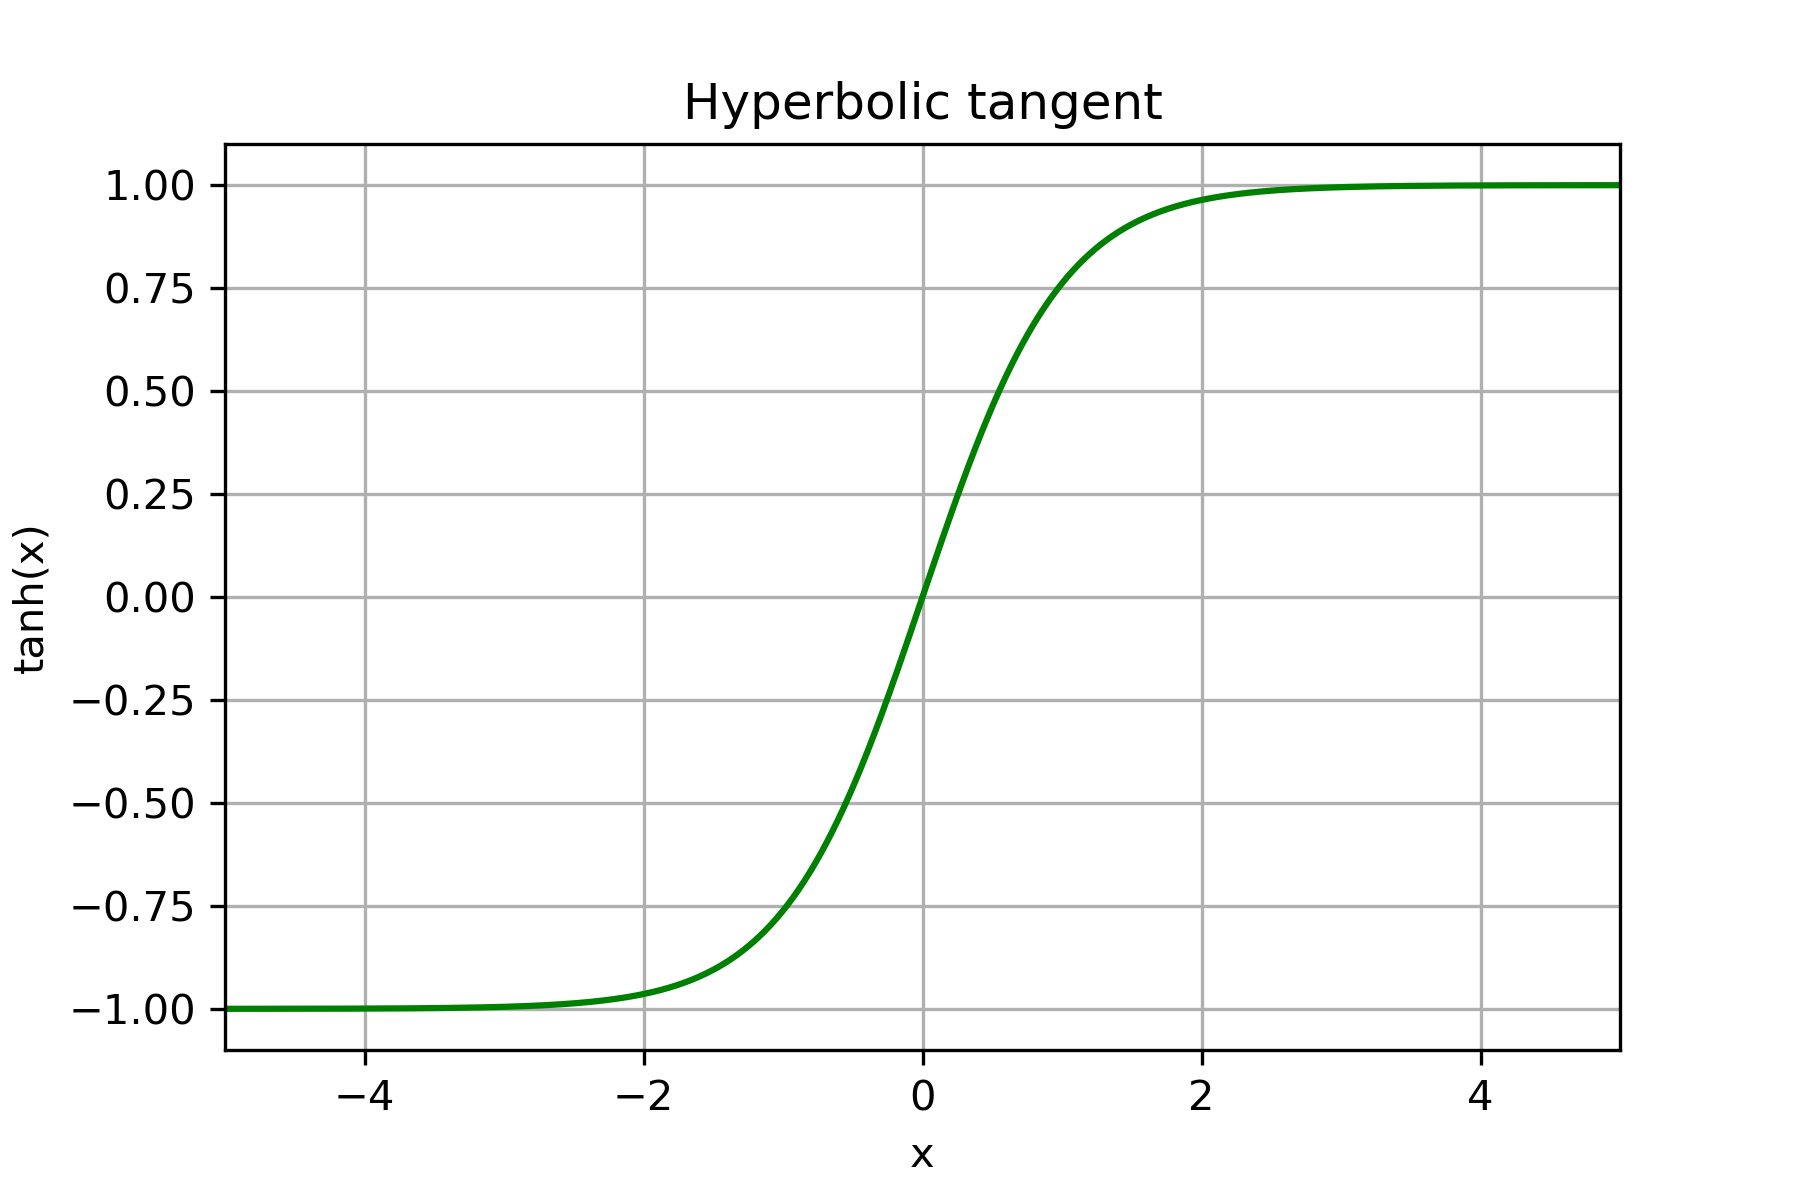
\includegraphics[width=12cm]{figure_0_hyperbolic_tangent}
    \caption{}
    \label{fig:pre-ex2-0}
\end{figure}

\paragraph{As we can see, the function is practically saturated for values smaller than -2.5 or bigger than 2.5. In fact, tanh(-3) returns -0.995 and tanh(3) returns 0.995. If we apply this function directly to the input data, almost all data would be under the saturated region. In order to avoid that, a linear transformation plus an offset was applied to all data. The goal is to work with the data in a region before the saturation region. It was chosen to work with the data in a range from -1 to 1. The figure \ref{fig:pre-ex2-1} shows the behavior of the hyperbolic tangent in this region.}

\begin{figure}[H]
    \centering
    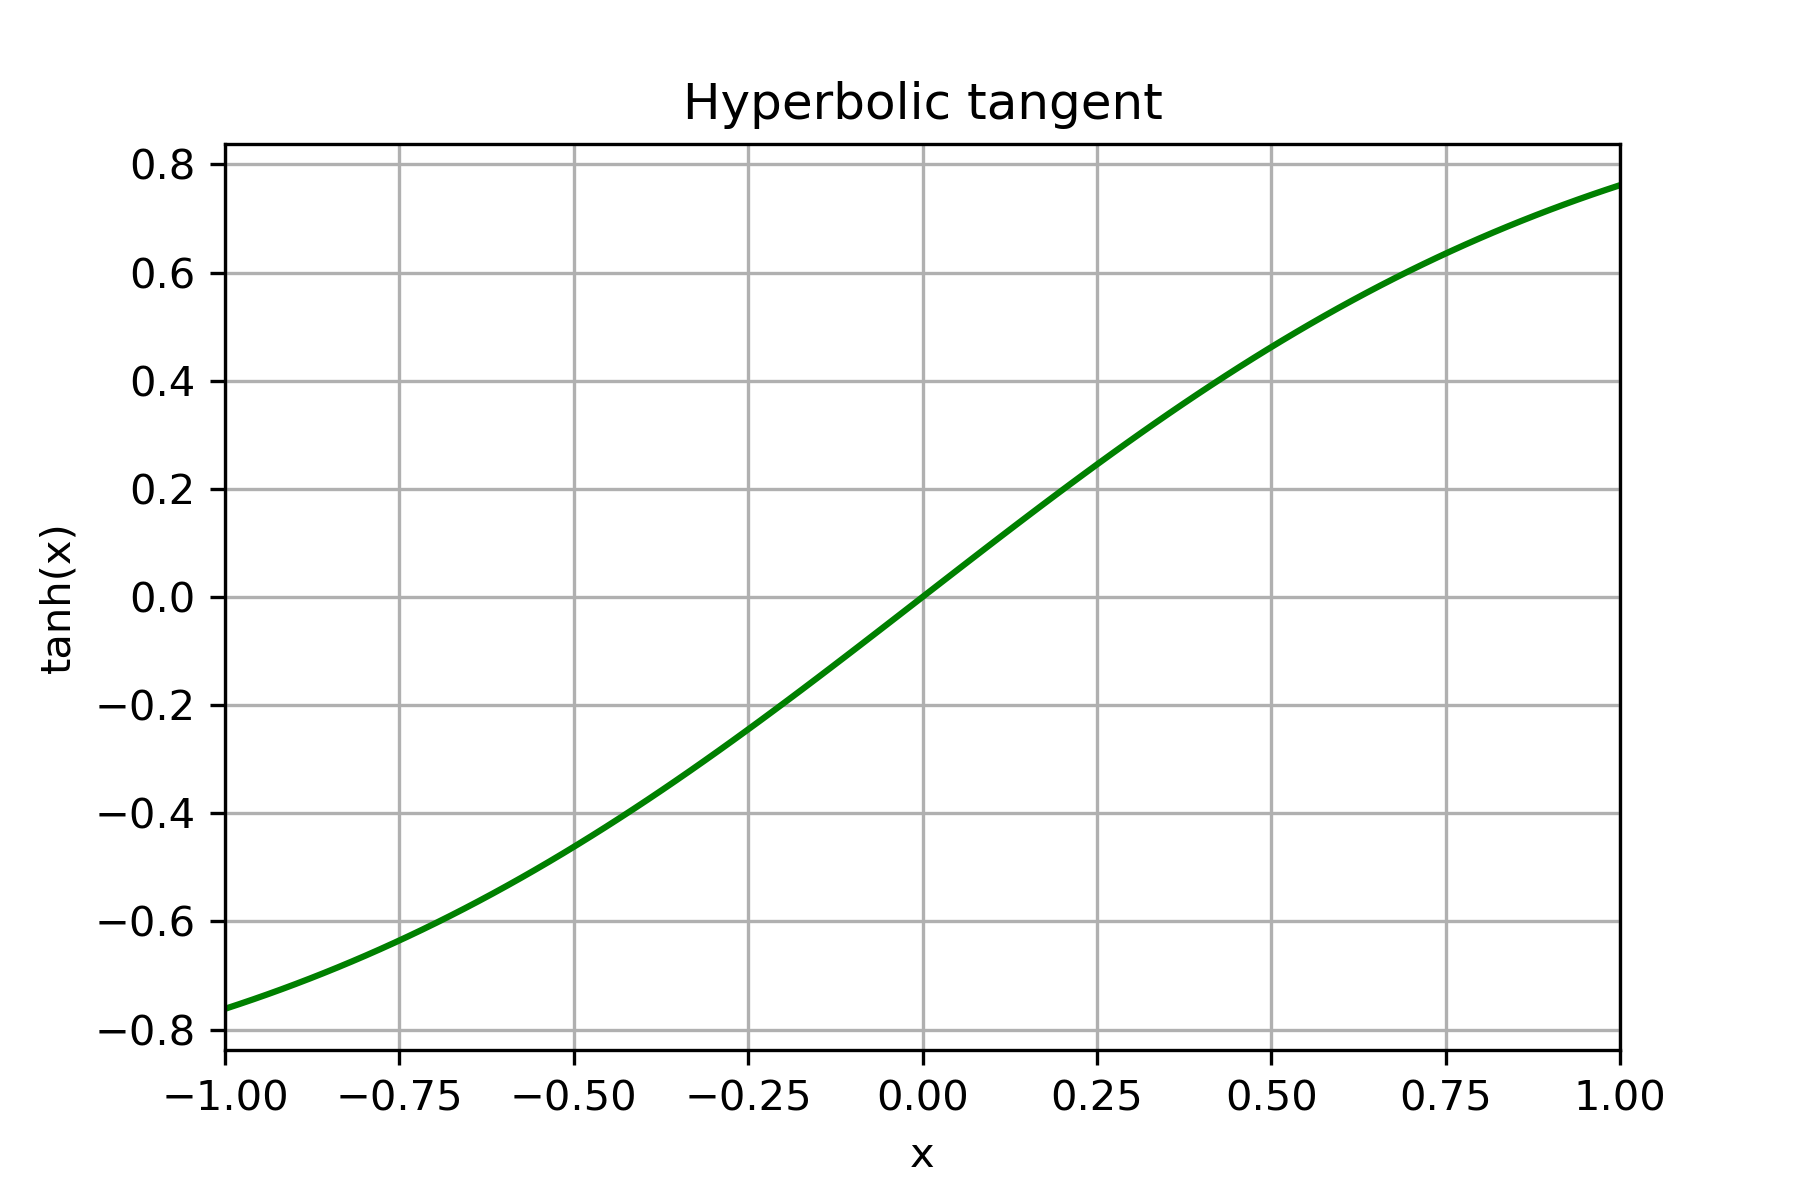
\includegraphics[width=12cm]{figure_1_hyperbolic_tangent}
    \caption{}
    \label{fig:pre-ex2-1}
\end{figure}

\paragraph{The procedure was to flatten the input data in a region from -1 to 1. To achieve this, we divided all data by the difference of the maximum and minimum input data, than applied a gain of 2 followed by an offset of -1. The first operation attenuated the data to be in the range of 0 to 1, the gain changed the range from 0 to 2 and the offset guaranteed the data to be in the range from -1 to 1. The figure \ref{fig:pre-ex2-2} shows the input data after this feature scaling and figure \ref{fig:pre-ex2-3} shows the data transformed after applying the hyperbolic tangent.}

\begin{figure}[H]
    \centering
    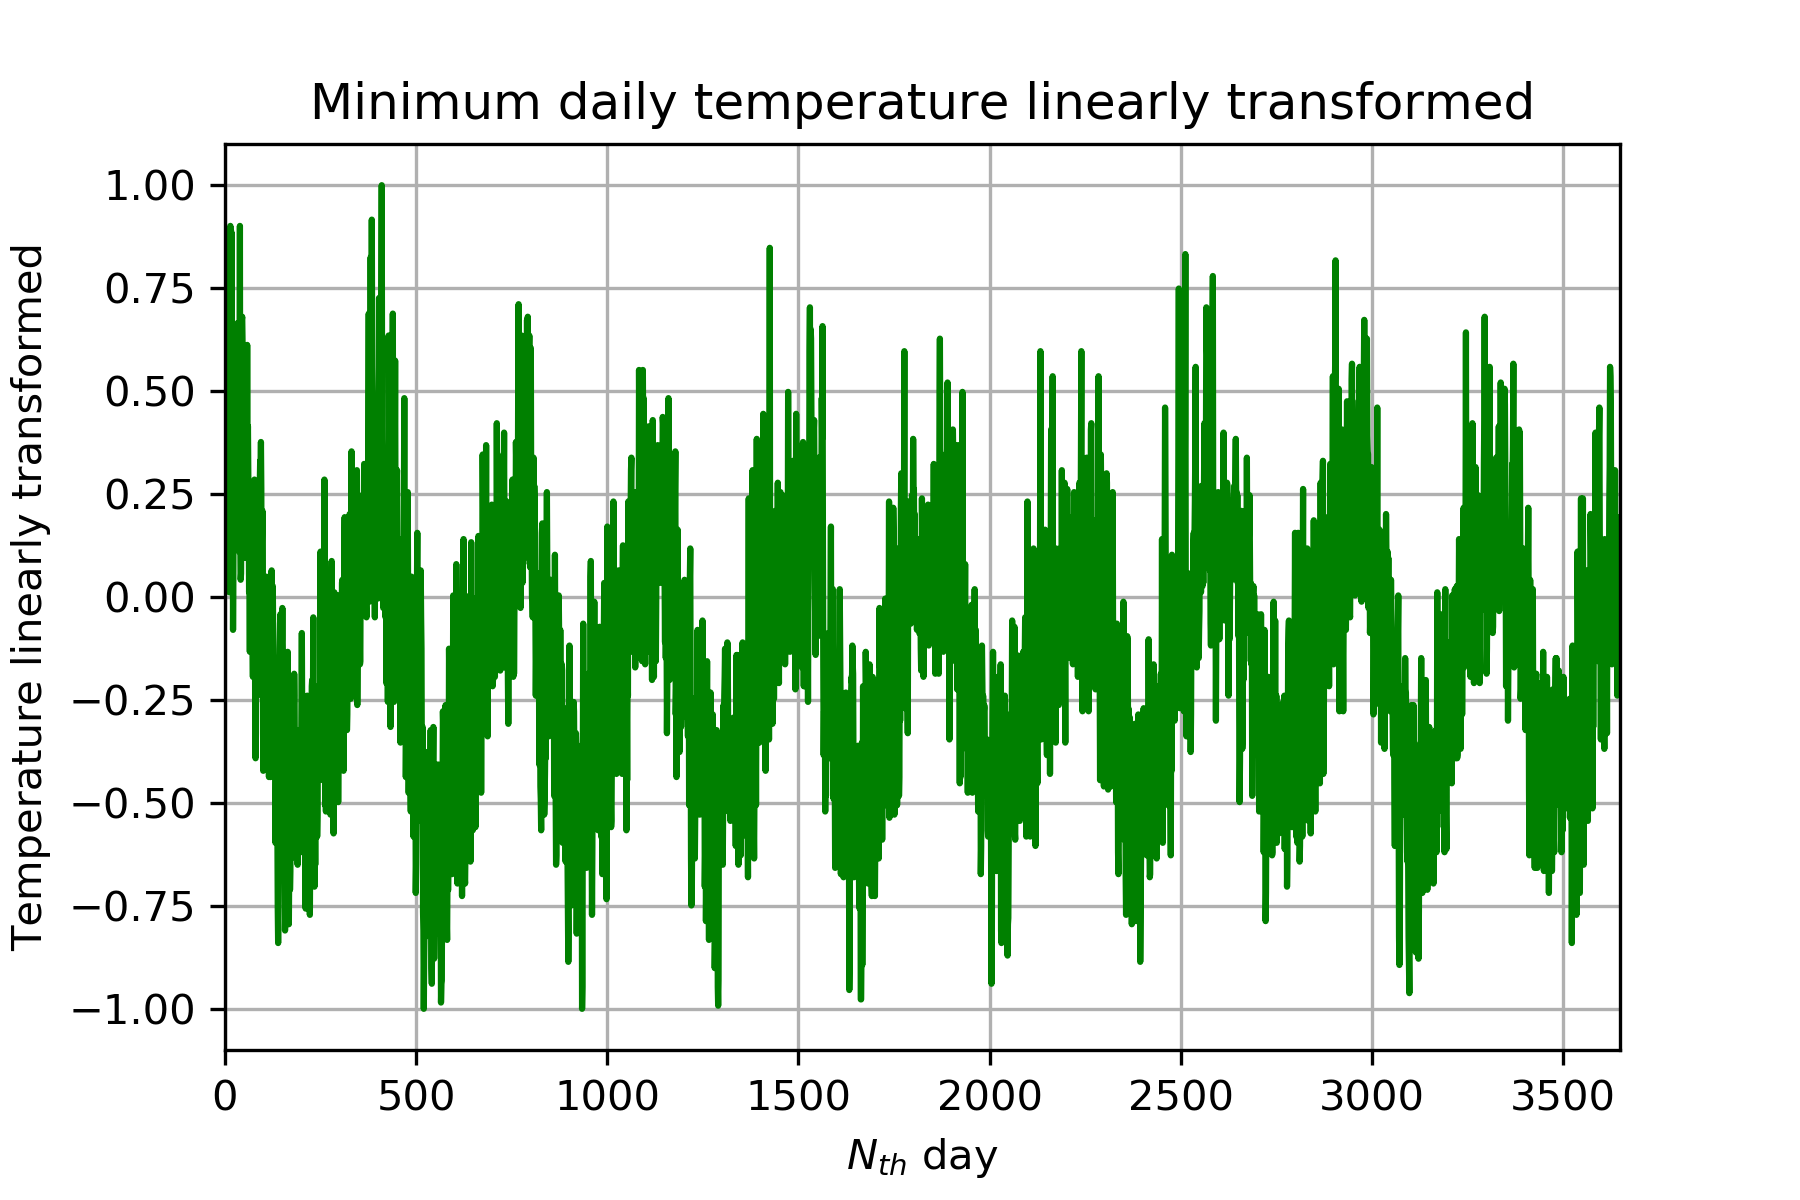
\includegraphics[width=12cm]{figure_2_linear_transformation}
    \caption{}
    \label{fig:pre-ex2-2}
\end{figure}

\begin{figure}[H]
    \centering
    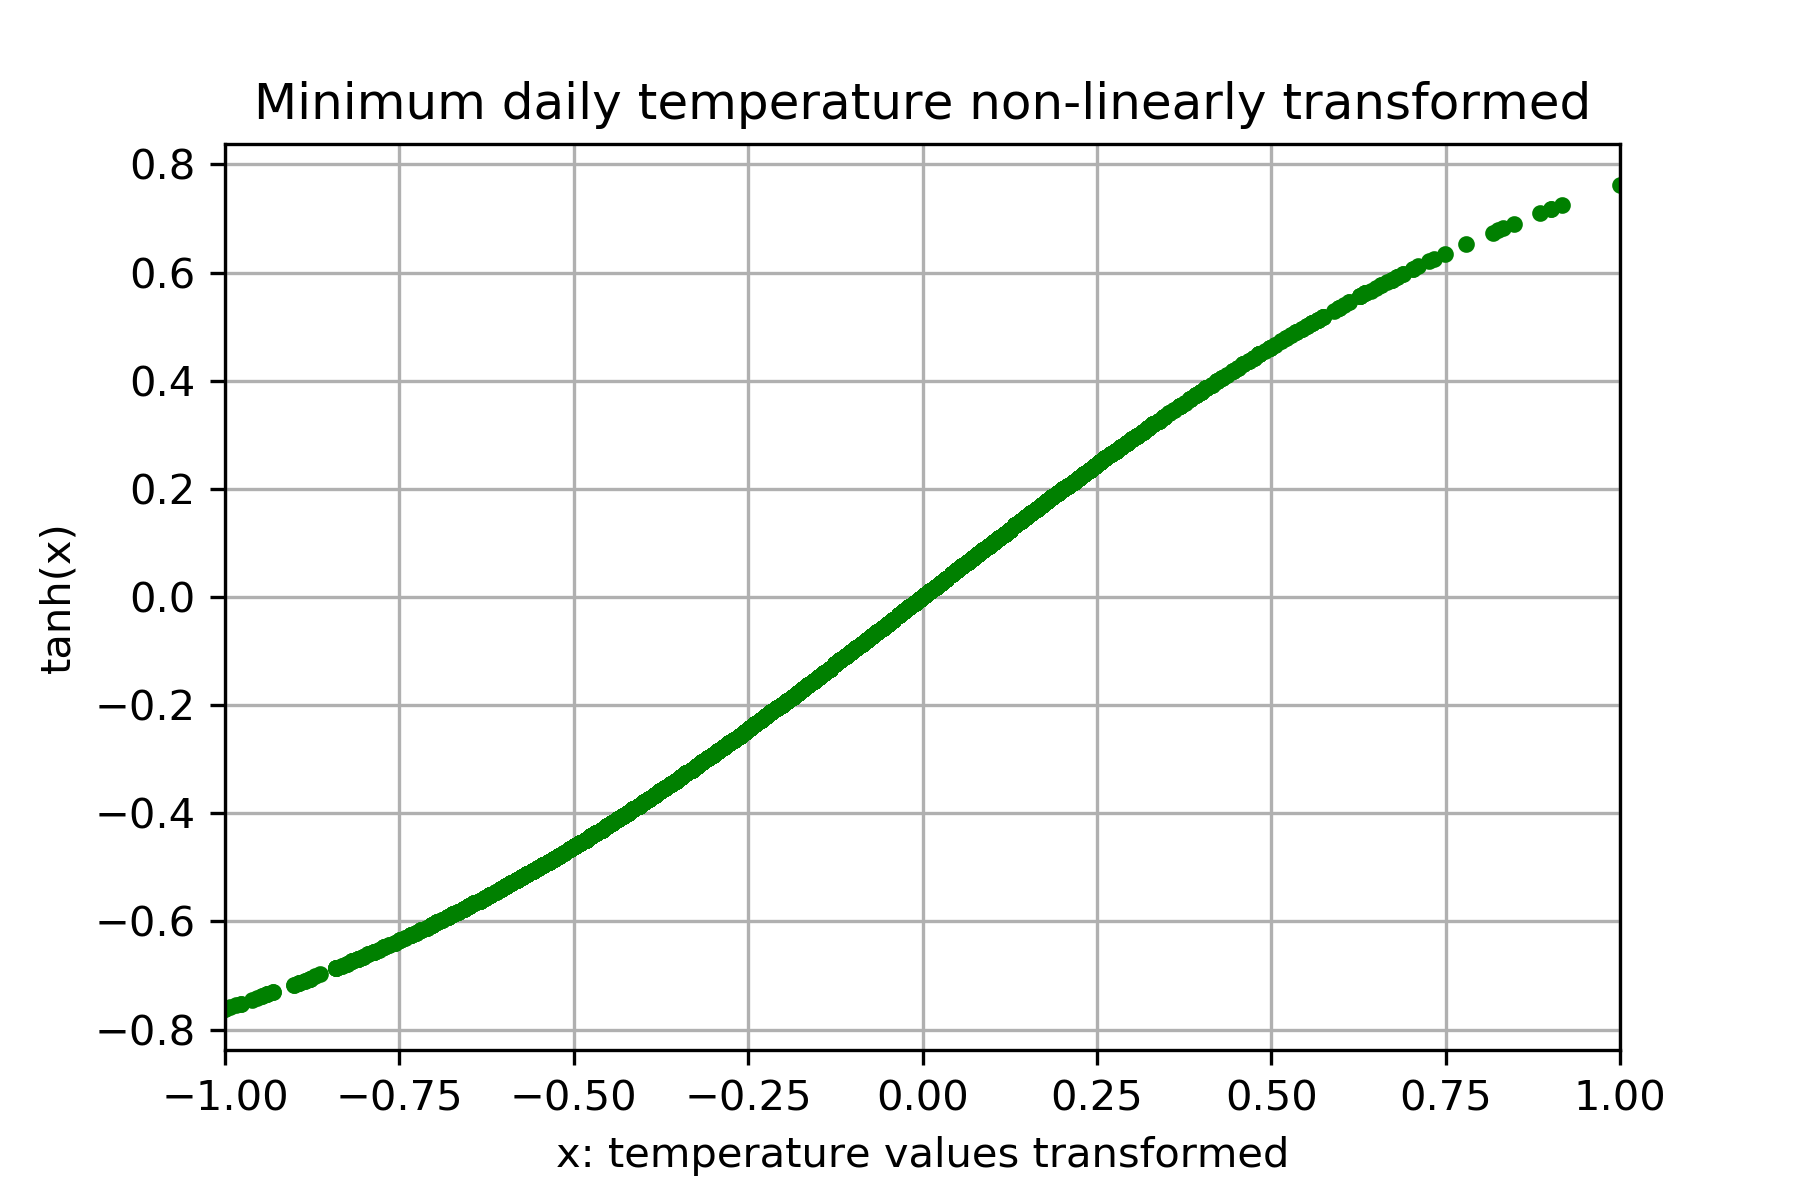
\includegraphics[width=12cm]{figure_3_tanh_dataset}
    \caption{}
    \label{fig:pre-ex2-3}
\end{figure}

%==============================
\subsubsection{a) Progression of the RMSE in function of the number of features T (from 1 to 100) taking K fixed to 5 days.}
%==============================

\paragraph{All functions used in the previous exercise were also utilized here. Additional functions were added in order to perform the feature scaling, to implement a one-dimensional golden-section search method (to find the best regularization coefficient) and a loop to train the model for each value of T.}

\paragraph{The model was trained for values of T from 1 to 100, and for each T a golden-section search was performed to find the optimum regularization coefficient. For this specific coefficient calculated for each T, the RMSE was measured. The progression of the root mean squared error measured with help of the k-fold cross-validation in the validation set can be seen in figure \ref{fig:ex2-1}.}

\begin{figure}[H]
    \centering
    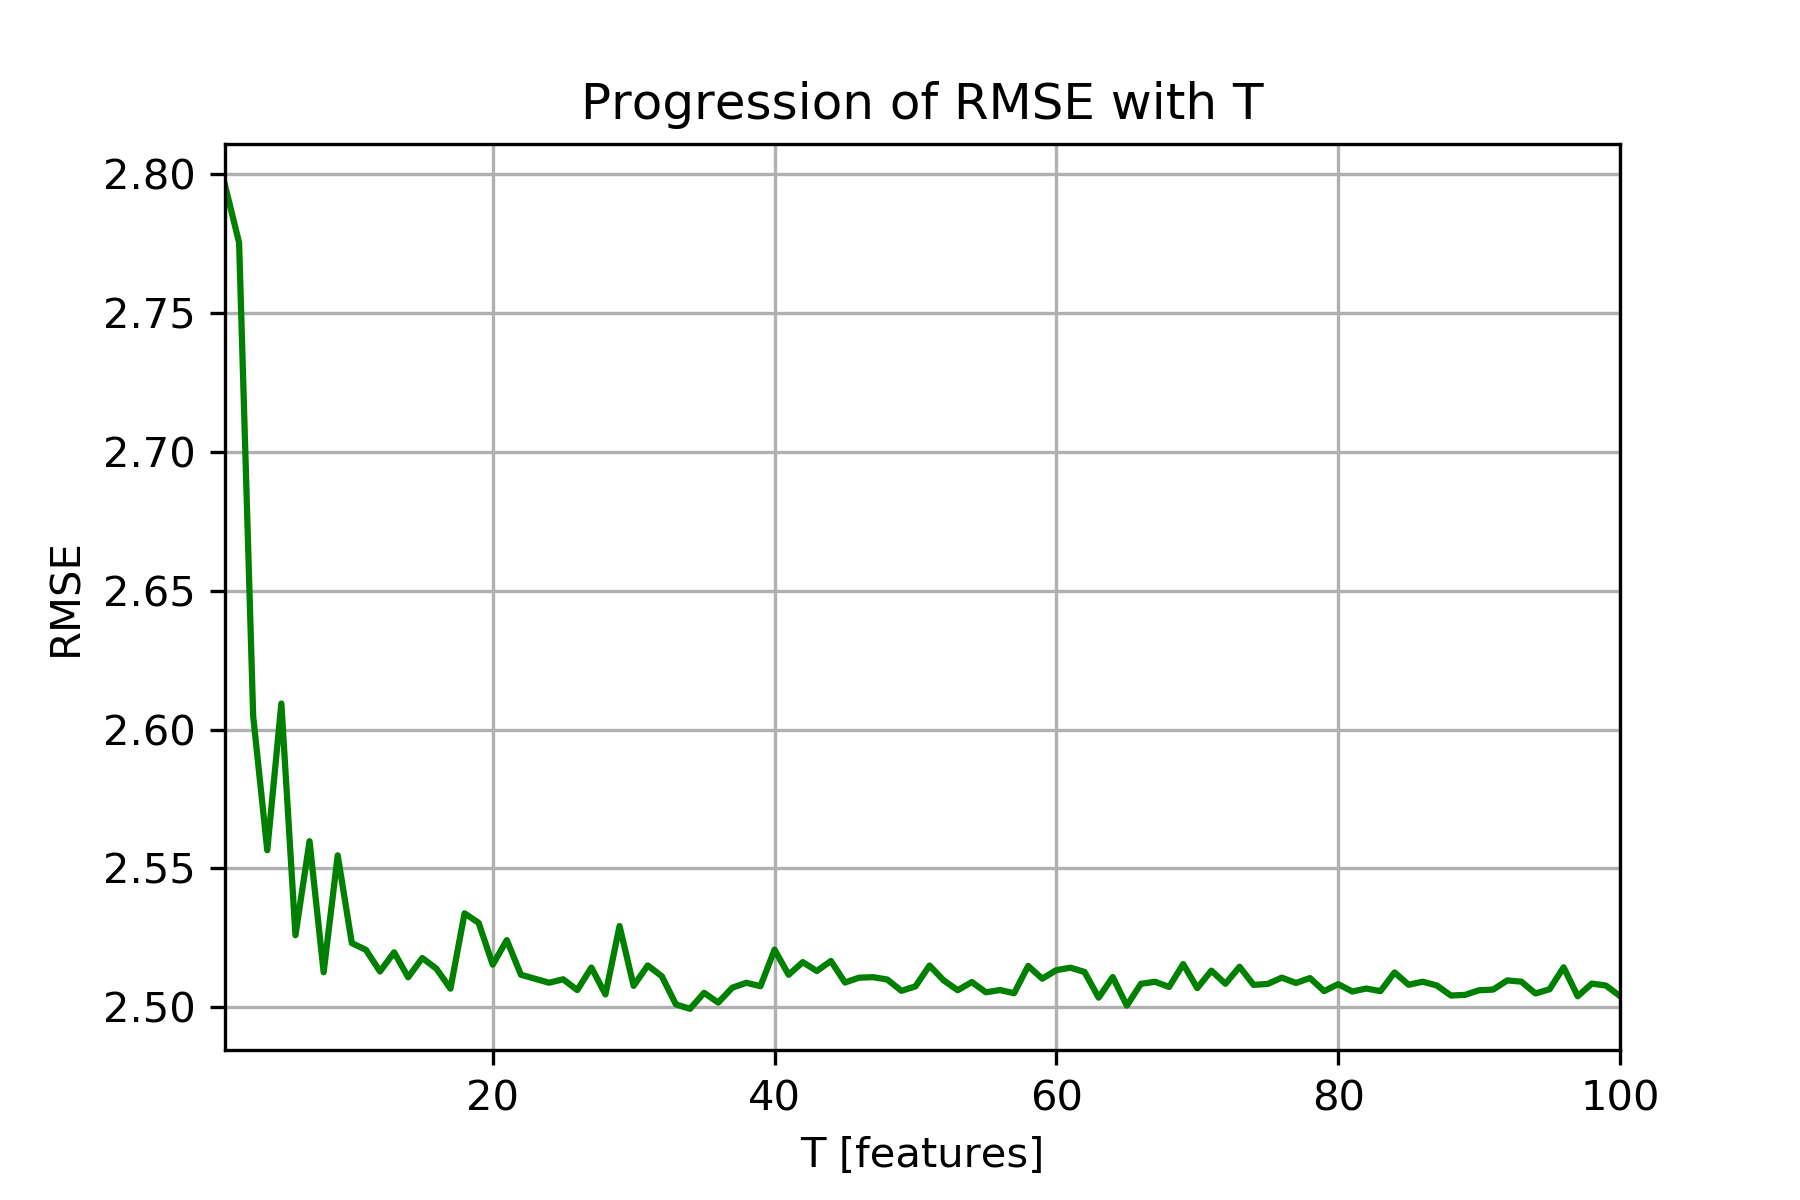
\includegraphics[width=12cm]{figure_1_rmse_with_T}
    \caption{}
    \label{fig:ex2-1}
\end{figure}

\paragraph{We can see a high value for the error for small T. After T equal to 10, the error seems to be more or less the same with a noisy added. In fact, the model was trained several times, and each time, the T for the smallest error changed. However, the range of this optimum T, was always in the same range: from 15 to 35. Also, the shape of the RMSE curve was also always the same: high error for small T, static with some noisy for T bigger than 20.
\\
For this specific case of training, we can zoom the previous figure and check that the T for the minimum error was 33. The fact of the optimum T keep changing for each model training is that for each training, the matrix wk is generated randomly and this randomness can interfere in the model. The curve for the RMSE zoomed can be seen in the figure \ref{fig:ex2-2}.}

\begin{figure}[H]
    \centering
    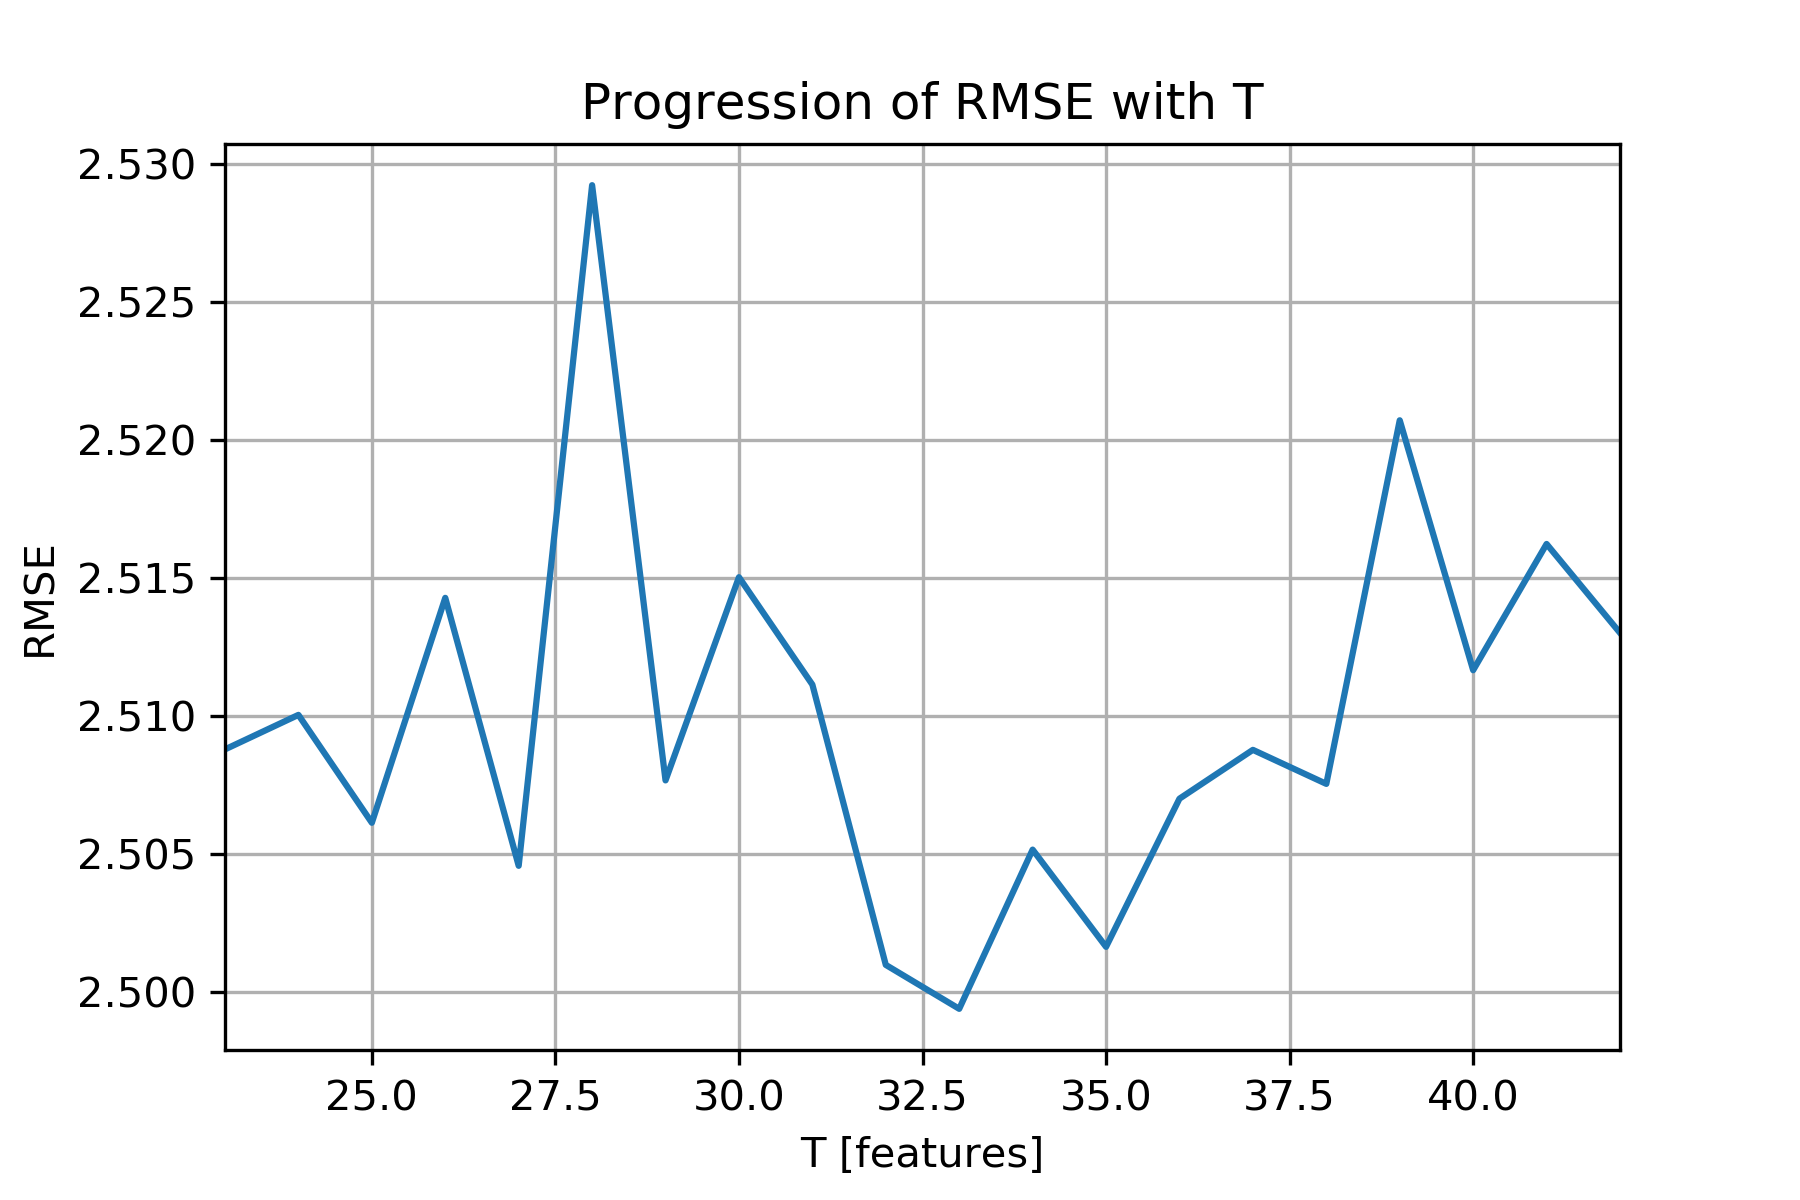
\includegraphics[width=12cm]{figure_2__rmse_with_T_zoom}
    \caption{}
    \label{fig:ex2-2}
\end{figure}

%==============================
\subsubsection{b) The best regularization coefficient for each value of T.}
%==============================

\paragraph{After having trained the model for each value of T, the optimum coefficient was saved to plot the next curve. The figure \ref{fig:ex2-3} shows the best lambda coefficient for each value of T. The regularization coefficient was found using a one-dimensional golden-section search method, searching in an interval of 1e-10 to 1e3 with a precision of 1e-12.}

\begin{figure}[H]
    \centering
    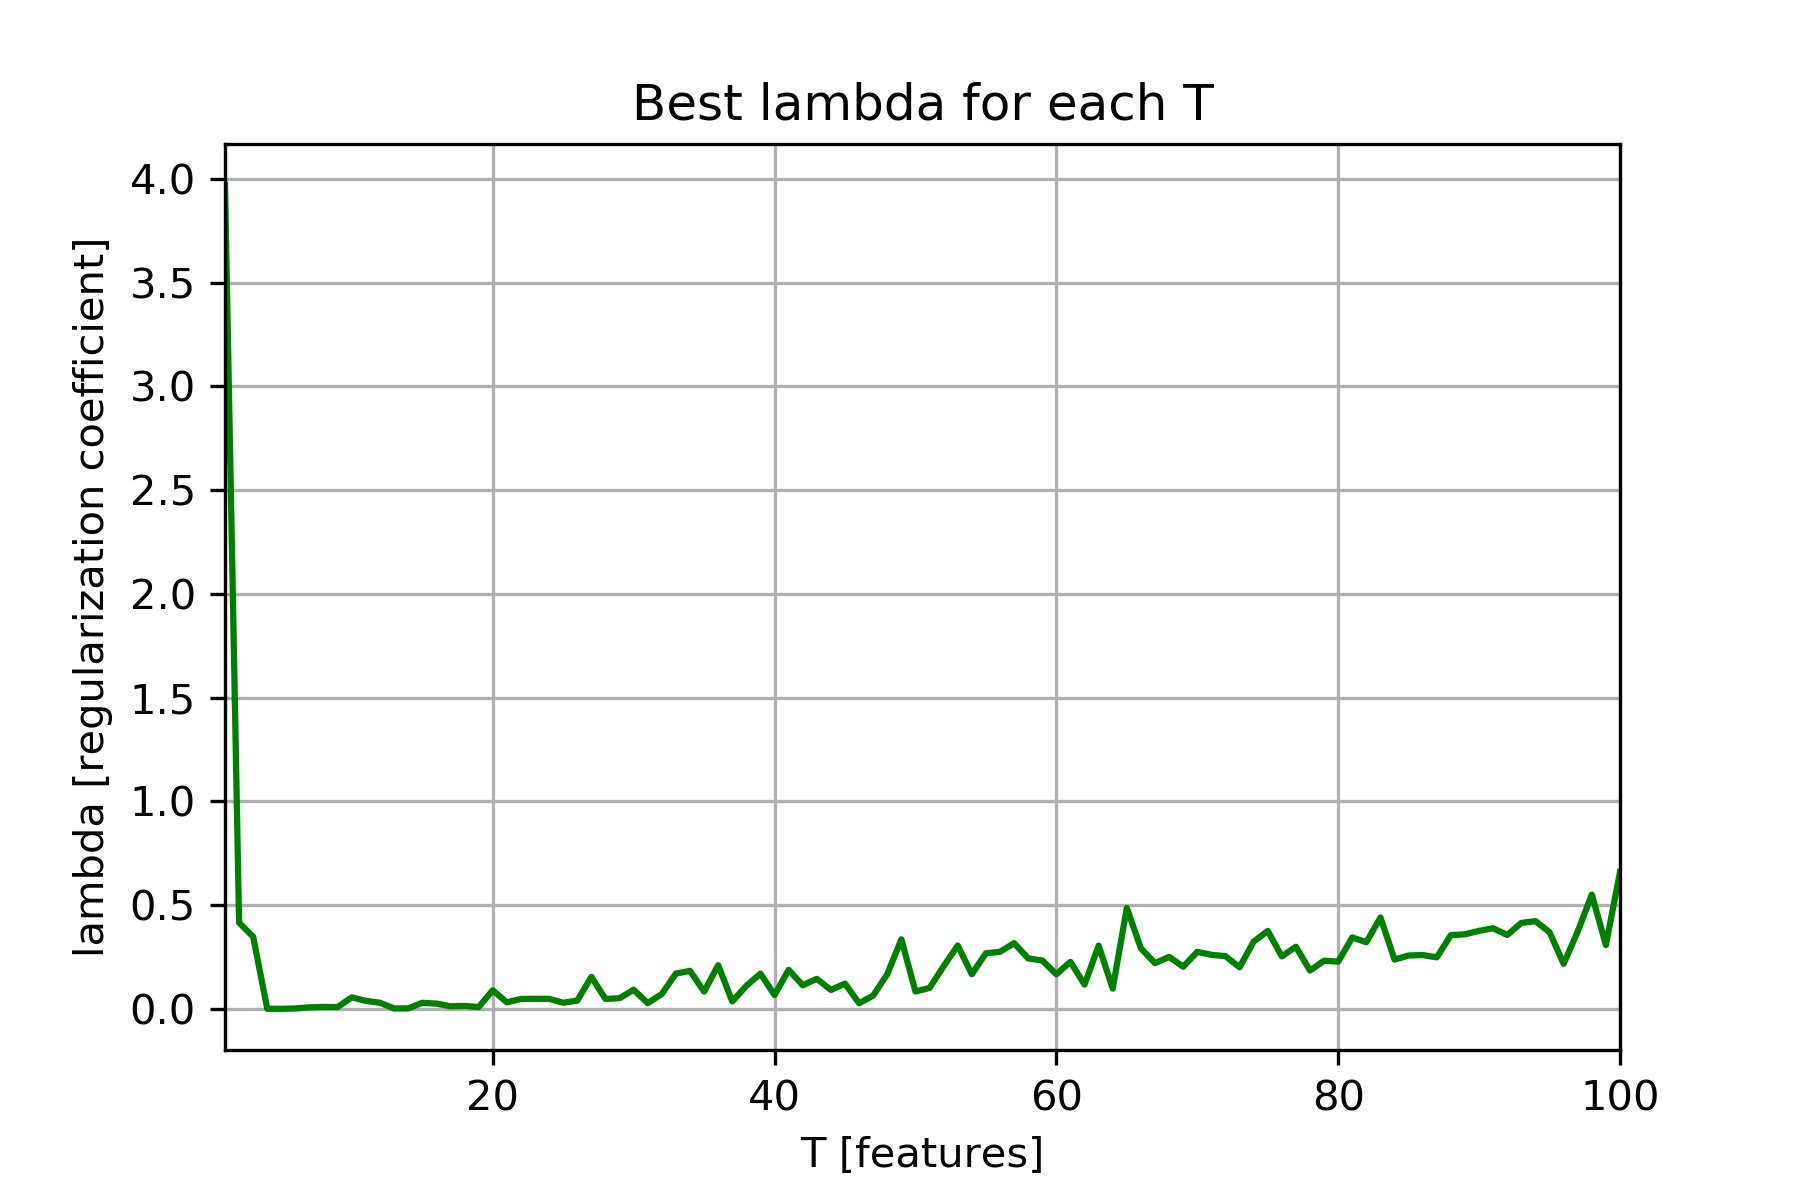
\includegraphics[width=12cm]{figure_3_lambda_with_T}
    \caption{}
    \label{fig:ex2-3}
\end{figure}

\paragraph{We can see that, with except of the very early values of T, when T increase, the optimum regularization coefficient, lambda, also increases. This means that when T increase, the model tends to penalty more and more the norm of weights array in order to try to reduce overfitting. In fact, for small values of T, lambda tends even to be zero, indicating that we are in a underfitting situation, or that trying to reduce the norm of the weights array is not so important.}

%==============================
\subsubsection{b) Plot the predicted and real temperatures of test set considering the best T and its corresponding regularization coefficient.}
%==============================

\paragraph{Now that we have the optimum T and also its optimum lambda, the model was trained with all data (i.e. not using cross-validation). The predicted minimum temperature and the real minimum temperature for the year of 1990 (test set) are plotted in the figure \ref{fig:ex2-4}.}

\begin{figure}[H]
    \centering
    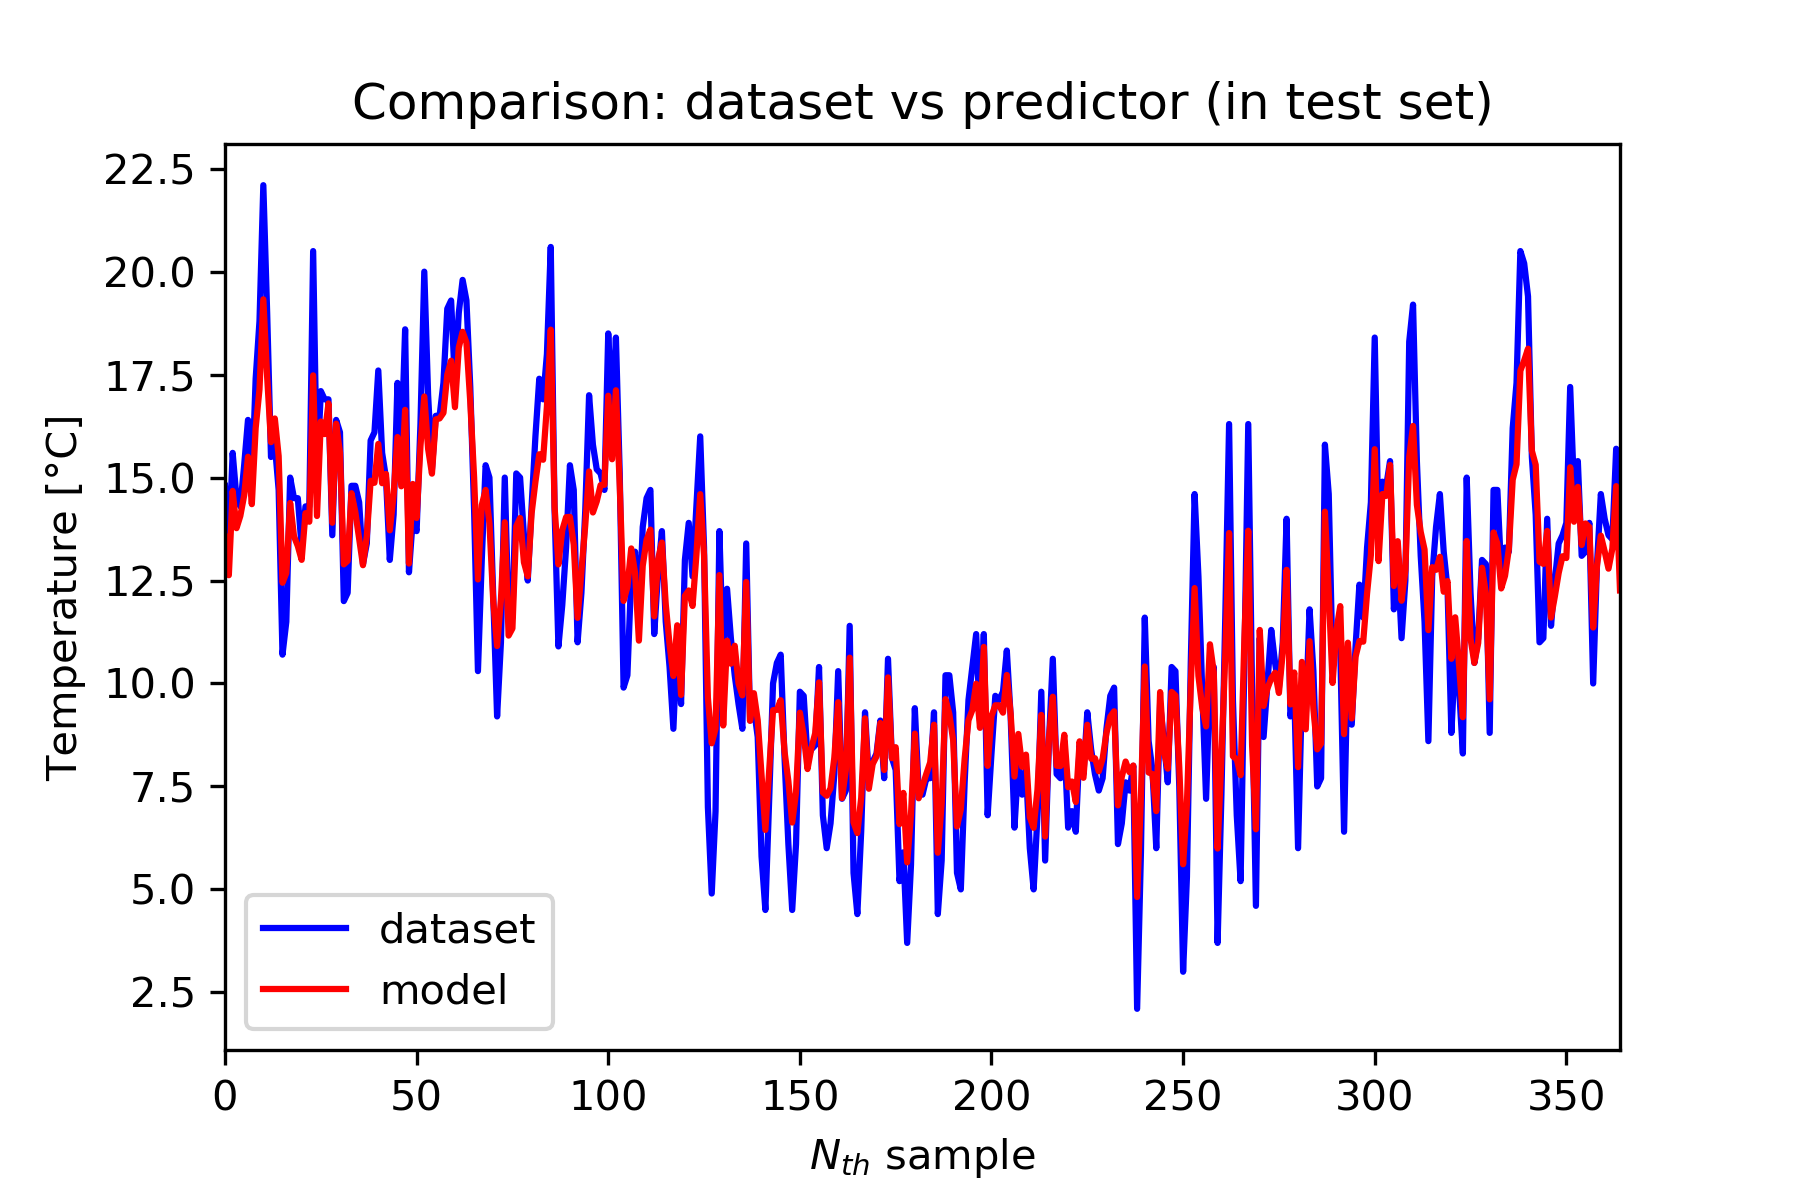
\includegraphics[width=12cm]{figure_4_predictor}
    \caption{}
    \label{fig:ex2-4}
\end{figure}

\paragraph{Despite the fact that each model training generates a new random matrix wk and this changes the best T chosen for that training, the RMSE calculated over the test year of 1990 does not change of magnitude. Several trainings were done, and the error always stayed in the range of 1.3 and 1.5. For the previous image, the RMSE calculated was 1.393, indicating that when a non-linear function is used, even though with random values for the wk matrix, a better result can be obtained from the linear regression of exercise 1.}

%=================================================
\end{document}
